%\documentclass[11pt,a4paper]{article}
\documentclass[11pt
  , a4paper
  , article
  , oneside
%  , twoside
%  , draft
]{memoir}

\usepackage{control}
\usepackage[numbers]{natbib}
\usepackage{graphicx,floatflt}

\begin{document}

\newcommand{\technumber}{
  RAON Control-Document Series\\
  Revision : v0.1,   Release : 2015.11.2}
\title{\textbf{KT Underground Laboratory Environment Monitoring System\\}}


\author{Seung Hee Nam\thanks{namsh@ibs.re.kr} \\
  Control Group \\
  Rare Isotope Science Project\\
  Institute for Basic Science\\
  Daejeon, South Korea
}

\date{\today}

\renewcommand{\maketitlehooka}{\begin{flushright}\textsf{\technumber}\end{flushright}}
%\renewcommand{\maketitlehookb}{\centering\textsf{\subtitle}}
%\renewcommand{\maketitlehookc}{C}
%\renewcommand{\maketitlehookd}{D}

\maketitle




\chapter{라즈베리파이 셋업}


KT 지하 실험실에 온습도 센서를 설치하기 전에 라즈베리 파이에 사용 할 수 있는 이미지를 생성하였다.
\begin{figure}[h]
	\begin{center}
		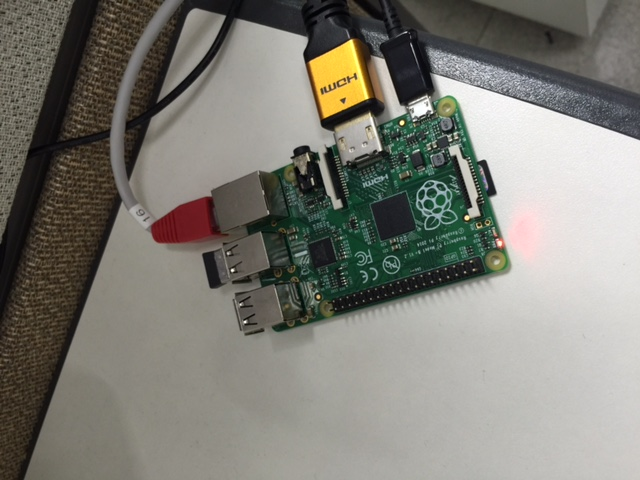
\includegraphics[width=7cm]{./images/1.JPG}
		\caption{RaspberryPi B+}
	\end{center}
\end{figure}

\subsection{Download raspbian image from}
\begin{lstlisting}[style=termstyle]
$ wget --content-disposition http://downloads.raspberrypi.org/raspbian_latest
$ unzip *raspbian*.zip
\end{lstlisting}
라즈비안을 다운받은후 압축을 풀어준다.
\subsection{Copy Image to SD Card}
\begin{lstlisting}[style=termstyle]
$ sudo dd bs=4M if=downloaded_image.img of=/dev/sdX
$ sync
$ umount /dev/sdX
\end{lstlisting}
dd를 이용해서 압축을 풀어준 라즈비안 이미지를 sd카드로 옮겨준다.\\
bs는 속도(4Mbyte)를 의미하고 if는 쓸 이미지 of는 쓰일위치이다.\\
쓰일 위치는 간단하게 df를 이용해서 확인할수있다.
\begin{lstlisting}[style=termstyle]
namsh@namsh:~/Downloads/icabu.2015.shn$ df -l
Filesystem                                              Size  Used Avail Use% Mounted on
rootfs                                                  184G   19G  156G  11% /
udev                                                     10M     0   10M   0% /dev
tmpfs                                                   1.6G  800K  1.6G   1% /run
/dev/disk/by-uuid/f4c99593-1541-478c-85df-8a2979a32cbc  184G   19G  156G  11% /
tmpfs                                                   5.0M     0  5.0M   0% /run/lock
tmpfs                                                   9.5G  185M  9.3G   2% /run/shm
/dev/sda1                                               487M  128K  486M   1% /boot/efi
/dev/sda4                                               1.6T   97G  1.5T   6% /home
\end{lstlisting}
\subsection{Insert SD Card to RaspberryPi and Expand User Partition}
PI 환경설정으로 아래와 같이 들어간후
\begin{lstlisting}[style=termstyle]
$ sudo rpi-config
\end{lstlisting}
1.Expand Filesystem을 해준뒤 리부팅 해준다.
\begin{lstlisting}[style=termstyle]
$ sudo reboot
\end{lstlisting}
\subsection{Network Configuration}
editor에는 자신이쓰는 에디터를 넣고 interfaces를 열어준다. (ex. nano, vi, emacs)
\begin{lstlisting}[style=termstyle]
$ sudo editor /etc/network/interfaces
\end{lstlisting}
쓸 ip address, netmask, gateway, dns-nameservers를 넣고 저장한다.
\begin{lstlisting}[style=termstyle]
iface eth0 inet static
address 10.1.4.206
netmask 255.255.255.0
gateway 10.1.4.254
dns-nameservers 10.1.2.240
\end{lstlisting}
무선 네트워크 설정은 다음과 같다.
\begin{lstlisting}[style=termstyle]
allow-hotplug wlan0
iface wlan0 inet static
address 10.1.4.??
netmask 255.255.255.0
gateway 10.1.4.254
dns-nameservers 10.1.2.240
wpa-scan-ssid 1
wpa-ap-ssid 1 
wpa-key-mgmt WPA-PSK
wpa-proto RSN WPA
wpa-pairwise CCMP TKIP
wpa-group CCMP TKIP
wpa-ssid "scwook"
wpa-psk "PASSWORD"
wpa-roam /etc/wpa_supplicant/wpa_supplicant.conf
iface default inet dhcp
\end{lstlisting}
pi 리부팅을 하거나 네트워크 리부팅을 해준다.
\begin{lstlisting}[style=termstyle]
$ sudo reboot
\end{lstlisting}
\begin{lstlisting}[style=termstyle]
$ sudo service network restart
\end{lstlisting}
\subsection{Package \& Firmware Upgrade}
아래와같이 패키지와 펌웨어 업데이트를 해준다.
\begin{lstlisting}[style=termstyle]
 $ sudo apt-get update
 $ sudo apt-get upgrade
 $ sudo rpi-update
\end{lstlisting}
\subsection{Setup GPIO}
라즈베리파이의 gpio를 사용하기위해서 wiringPi를 설치 해준다.
\begin{lstlisting}[style=termstyle]
 $ git clone git://git.drogon.net/wiringPi
 $ cd wiringPi
 $ sudo ./build
\end{lstlisting}
\subsection{Download and Install EPICS}
EPICS를 다운받을 위치로 이동 후 EPICS 스크립트를 다운받고 루트계정으로 접속한다.
\begin{lstlisting}[style=termstyle]
 $ git clone https://github.com/jeonghanlee/scripts_for_epics.git
 $ ~$ cd scripts_for_epics/  
 $ ~/scripts_for_epics$ sudo su
 Password: 
\end{lstlisting}
Pi에 EPICS를 설치하기위해서는 lsb\_release가 필요하므로 설치해준다.
\begin{lstlisting}[style=termstyle]
$ root@:{HOME}/scripts_for_epics# aptitude install lsb_release
\end{lstlisting}
require\_package 부터 설치한뒤 EPICS를 설치해준다.\\
설치가 끝나면 epics/R3.14.12.5/에 들어가 . setEpicsEnv를 해준다.
\begin{lstlisting}[style=termstyle]
$ root@:{HOME}/scripts_for_epics# bash require_packages.sh all
$ root@:{HOME}/scripts_for_epics# exit
$ ~/scripts_for_epics$ bash epics_default_installation.sh 
$ ~/scripts_for_epics$ cd ../epics/R3.14.12.5/
$ ~/epics/R3.14.12.5$ ls
base  extensions  setEpicsEnv.sh
$ ~/epics/R3.14.12.5$ . setEpicsEnv.sh 
\end{lstlisting}
\subsection{Download siteApp and siteLib}
아래와 같은 스크립트를 실행시켜 필요 앱과 라이브러리를 다운받는다.
\begin{lstlisting}[style=termstyle]
 $ ~/scripts_for_epics$ bash raon_cloning.sh
\end{lstlisting}
\subsection{Build an image of configured rPi and copy it to new SD casd}
dd를 이용하여 SD카드에 설치한 라즈비안과 이외의 패키지를 이미지화 시킨다.
\begin{lstlisting}[style=termstyle]
 $ sudo dd bs=4M if=name_of_new_image.img if=/dev/sd?
 $ sync
\end{lstlisting}
차후 이렇게 만든 이미지 파일은 새로운 파이를 만들때 따로 설정할 필요없이 이미지만 dd를 이용해서 옮김으로 편리하게 새로운 Pi를 만들수 있는 강점이 있다.
\begin{lstlisting}[style=termstyle]
$ sudo dd bs=4M if=/dev/sd? of=name_of_new_image.img
\end{lstlisting}
아래와같이 새로운 SD카드에 이미지를 쓰면 이전과 똑같은 Pi가 만들어진다.
\begin{lstlisting}[style=termstyle]
 $ sudo dd bs=4M if=name_of_new_image.img if=/dev/sd?
 $ sync
\end{lstlisting}
\subsection{Auto reconnection wireless LAN}
무선인터넷 사용중 무선인터넷에 끊김이 발생할때 파이는 자동으로 무선인터넷을 잡아주지 않기 때문에 다시 접속하여 사용해야한다. 이런 불편을 없애려면 아래와 같은 코드를 추가해 주어야한다.
\begin{lstlisting}[style=termstyle]
$ cd /etc/ifplugd/action.d/
$ sudo mv ifupdown ifupdown.original
$ sudo cp /etc/wpa_supplicant/ifupdown.sh ./ifupdown
$ sudo reboot
\end{lstlisting}

\subsection{SHT71센서 설정}
이미 SHT71 센서에 대한 integration은 제어 그룹의 손창욱 연구원이 완료한 상태이기 때문에 기본적인 설정을 하면 센서를 사용할 수 있다.
RaonControl.git에서 받은 siteLibs와 siteApps를 이용하면 되는데 모든 라이브러리를 컴파일 할 필요가 없으므로 siteLibs/RPiLibPack/SHT7xSrc에서 make를 해주면 siteApps의 IOC를 사용하기 위한 준비를 마칠수 있다.
\begin{lstlisting}[style=termstyle]
namsh@namsh:~/epics/R3.14.12.5/siteLibs/RPiLibPack/src/SHT7xSrc$ make
perl /home/namsh/epics/R3.14.12.5/base/bin/linux-x86_64/makeMakefile.pl O.linux-x86_64 ../../../..
mkdir O.Common
make -C O.linux-x86_64 -f ../Makefile TOP=../../../.. \
T_A=linux-x86_64 install
make[1]: Entering directory `/home/namsh/epics/R3.14.12.5/siteLibs/RPiLibPack/src/SHT7xSrc/O.linux-x86_64'
Installing dbd file /home/namsh/epics/R3.14.12.5/siteLibs/dbd/shtRecord.dbd
mkdir /home/namsh/epics/R3.14.12.5/siteLibs/dbd
Installing dbd file /home/namsh/epics/R3.14.12.5/siteLibs/dbd/devSHT7x.dbd
echo "../O.Common/shtRecord.h : ../Makefile" >> shtRecord.h.d
/home/namsh/epics/R3.14.12.5/base/bin/linux-x86_64/dbToRecordtypeH   -I. -I.. -I../O.Common -I/home/namsh/epics/R3.14.12.5/siteLibs/dbd -I/home/namsh/epics/R3.14.12.5/base/dbd ../shtRecord.dbd shtRecord.h
Installing generated generic include file /home/namsh/epics/R3.14.12.5/siteLibs/include/shtRecord.h
mkdir /home/namsh/epics/R3.14.12.5/siteLibs/include

/usr/bin/gcc -c  -D_GNU_SOURCE -D_DEFAULT_SOURCE            -D_X86_64_  -DUNIX  -Dlinux     -O3 -g   -Wall       -m64     -fPIC -MMD -I. -I../O.Common -I. -I.. -I/home/namsh/epics/R3.14.12.5/siteLibs/include/os/Linux -I/home/namsh/epics/R3.14.12.5/siteLibs/include -I/home/namsh/epics/R3.14.12.5/base/include/os/Linux -I/home/namsh/epics/R3.14.12.5/base/include        ../RPi_SHT1x.c 
In file included from ../RPi_SHT1x.c:14:0:
../RPi_SHT1x.h:18:22: fatal error: wiringPi.h: No such file or directory
compilation terminated.
\end{lstlisting}
컴파일이 끝나면 siteApps/raspberry/sht7xApp으로 들어가서 다시한번 make를 하면 IOC를 사용할 수 있다.
\begin{lstlisting}[style=termstyle]
namsh@namsh:~/epics/R3.14.12.5/siteApps/raspberry/sht7xApp$ make
make -C ./src install 
make[1]: Entering directory `/home/namsh/epics/R3.14.12.5/siteApps/raspberry/sht7xApp/src'
perl /home/namsh/epics/R3.14.12.5/base/bin/linux-x86_64/makeMakefile.pl O.linux-x86_64 ../../..
mkdir O.Common
make -C O.linux-x86_64 -f ../Makefile TOP=../../.. \
T_A=linux-x86_64 install
make[2]: Entering directory `/home/namsh/epics/R3.14.12.5/siteApps/raspberry/sht7xApp/src/O.linux-x86_64'
perl /home/namsh/epics/R3.14.12.5/base/bin/linux-x86_64/makeIncludeDbd.pl base.dbd shtRecord.dbd devSHT7x.dbd sht7xInclude.dbd
echo "../O.Common/sht7xInclude.dbd : ../Makefile" >> sht7x.dbd.d
Expanding dbd
Installing created dbd file ../../../dbd/sht7x.dbd
mkdir ../../../dbd
perl /home/namsh/epics/R3.14.12.5/base/bin/linux-x86_64/registerRecordDeviceDriver.pl ../O.Common/sht7x.dbd sht7x_registerRecordDeviceDriver /home/namsh/epics/R3.14.12.5/siteApps/raspberry > sht7x.tmp
mv sht7x.tmp sht7x_registerRecordDeviceDriver.cpp

/usr/bin/g++ -c  -D_GNU_SOURCE -D_DEFAULT_SOURCE            -D_X86_64_  -DUNIX  -Dlinux     -O3 -g   -Wall       -m64      -MMD -I. -I../O.Common -I. -I.. -I../../../include/os/Linux -I../../../include  -I/home/namsh/epics/R3.14.12.5/epicsLibs/synApps_5_8/support/seq-2-2-1/include -I/home/namsh/epics/R3.14.12.5/base/include/os/Linux -I/home/namsh/epics/R3.14.12.5/base/include  -I/home/namsh/epics/R3.14.12.5/epicsLibs/synApps_5_8/support/asyn-4-26/include  -I/home/namsh/epics/R3.14.12.5/epicsLibs/synApps_5_8/support/stream-2-6a/include     -I/home/namsh/epics/R3.14.12.5/siteLibs/include -I/home/namsh/epics/R3.14.12.5/extensions/include -I/home/pi/wiringPi/wiringPi    sht7x_registerRecordDeviceDriver.cpp 

/usr/bin/g++ -c  -D_GNU_SOURCE -D_DEFAULT_SOURCE            -D_X86_64_  -DUNIX  -Dlinux     -O3 -g   -Wall       -m64      -MMD -I. -I../O.Common -I. -I.. -I../../../include/os/Linux -I../../../include  -I/home/namsh/epics/R3.14.12.5/epicsLibs/synApps_5_8/support/seq-2-2-1/include -I/home/namsh/epics/R3.14.12.5/base/include/os/Linux -I/home/namsh/epics/R3.14.12.5/base/include  -I/home/namsh/epics/R3.14.12.5/epicsLibs/synApps_5_8/support/asyn-4-26/include  -I/home/namsh/epics/R3.14.12.5/epicsLibs/synApps_5_8/support/stream-2-6a/include     -I/home/namsh/epics/R3.14.12.5/siteLibs/include -I/home/namsh/epics/R3.14.12.5/extensions/include -I/home/pi/wiringPi/wiringPi    ../sht7xMain.cpp 
make[2]: *** No rule to make target `/home/namsh/epics/R3.14.12.5/siteLibs/lib/linux-x86_64/libraspSHT7x.a', needed by `sht7x'.  Stop.
make[2]: Leaving directory `/home/namsh/epics/R3.14.12.5/siteApps/raspberry/sht7xApp/src/O.linux-x86_64'
\end{lstlisting}
IOC는 siteApps/raspberry/iocBoot/iocRaspberryPi의 st.cmd.sht7x를 실행하면 된다.
\begin{lstlisting}[style=termstyle]

\end{lstlisting}
\chapter{모니터링 파이용 케이스 디자인}
모니터링 파이용 케이스를 만들기 위해서 스케치업 3D 툴을 이용하였고 Archiver Appliance를 이용해 온도와 습도 값을 저장하였다 그리고 통계프로그램인 R을 이용해서 온도의 오차나 경향성을 확인하고 분석했다.
\section{스케치업과 R을 이용한 케이스 디자인}
스케치업을 통해서 디자인한 케이스는 Version1~8까지 7번의 디자인 변경이 있었고 version8은 version7 케이스의 테스트가 끝난뒤 디자인되어 현재 적용된 케이스는 version7 케이스이다.
케이스를 디자인하며 케이스안에 있는 센서가 믿을 만한지 알기 위해서 통계 프로그램 R을 이용하여 내부의 센서와 외부의 센서 값을 비교하였으며 이를 통해 케이스 디자인을 점차적으로 업그레이드 시켰다.
R을 이용해서 plot을 하기 위해서 python scrip를 통해서 아카이빙된 데이터를 txt형식으로 저장했으며 이를 plot했다.\\
데이터를 txt형식으로 바꾸기위한 getData.py 스크립트는 이정한 박사님이 작성하였으며 여러가지 옵션에 따라 데이터를 저장할수 있도록 되어있다. 자세한 사항은 scripts\_for\_epics/\\archiver.appliance.python의 getData.py를 참조하면 된다.
\begin{center}
	\begin{figure}[h]
		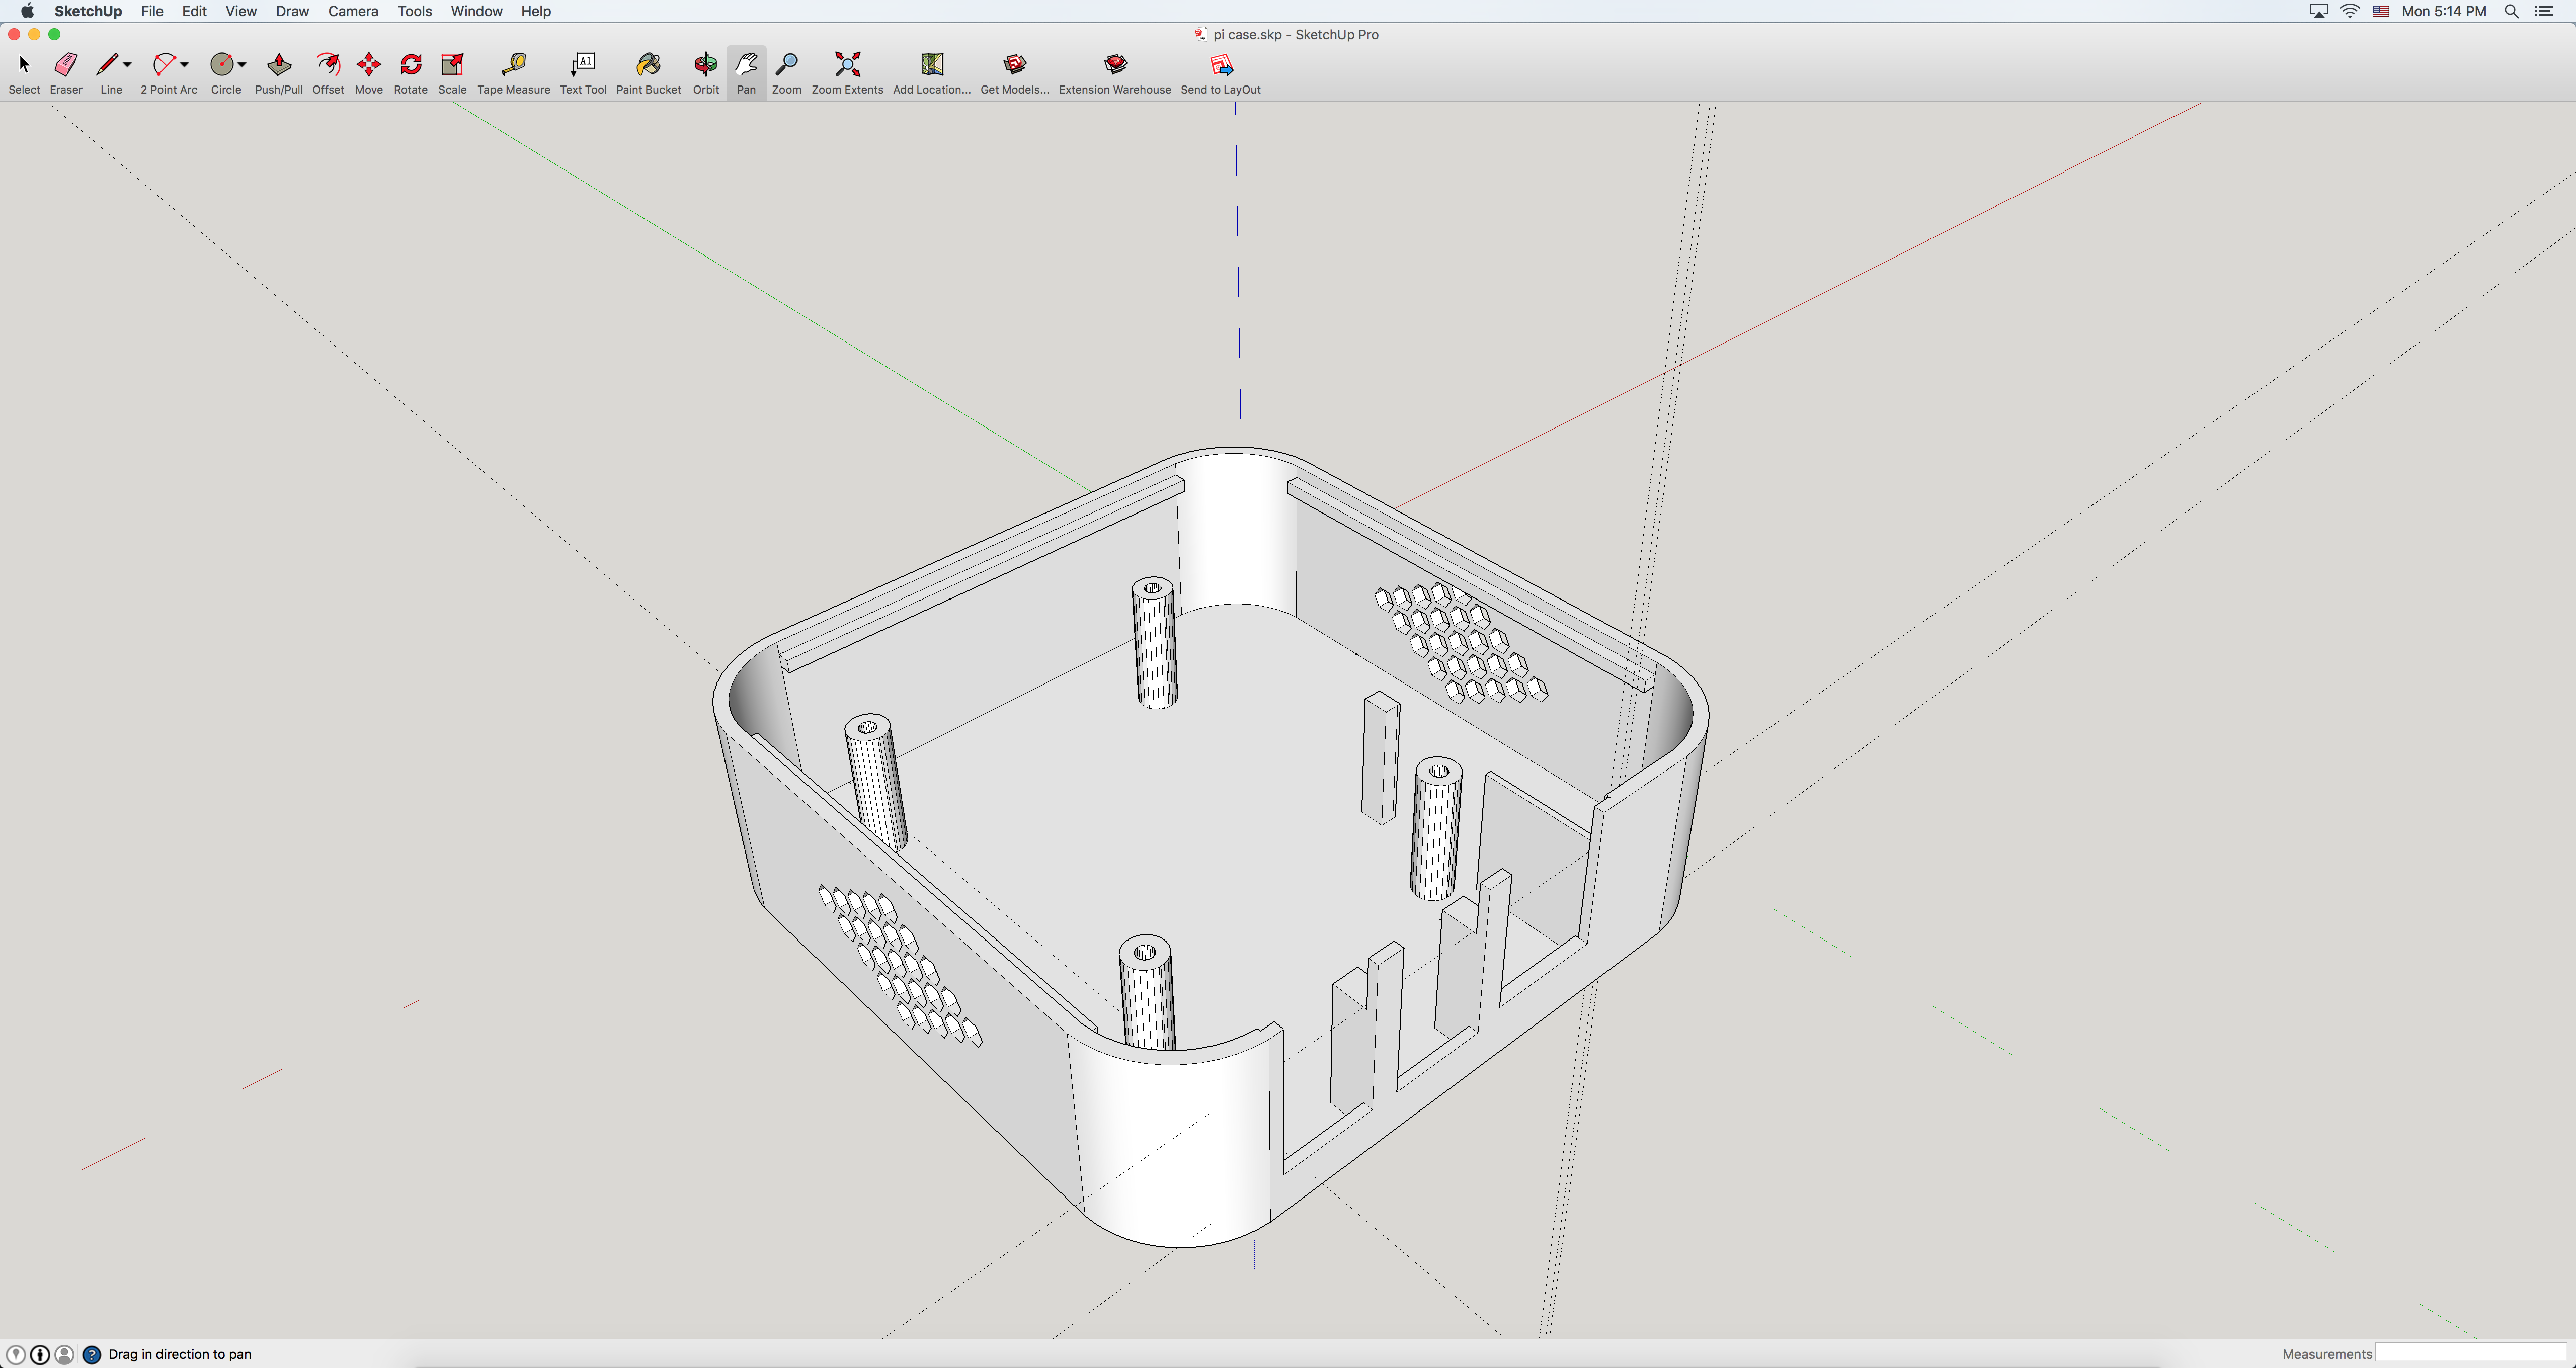
\includegraphics[width=8cm]{./images/V1.png}
		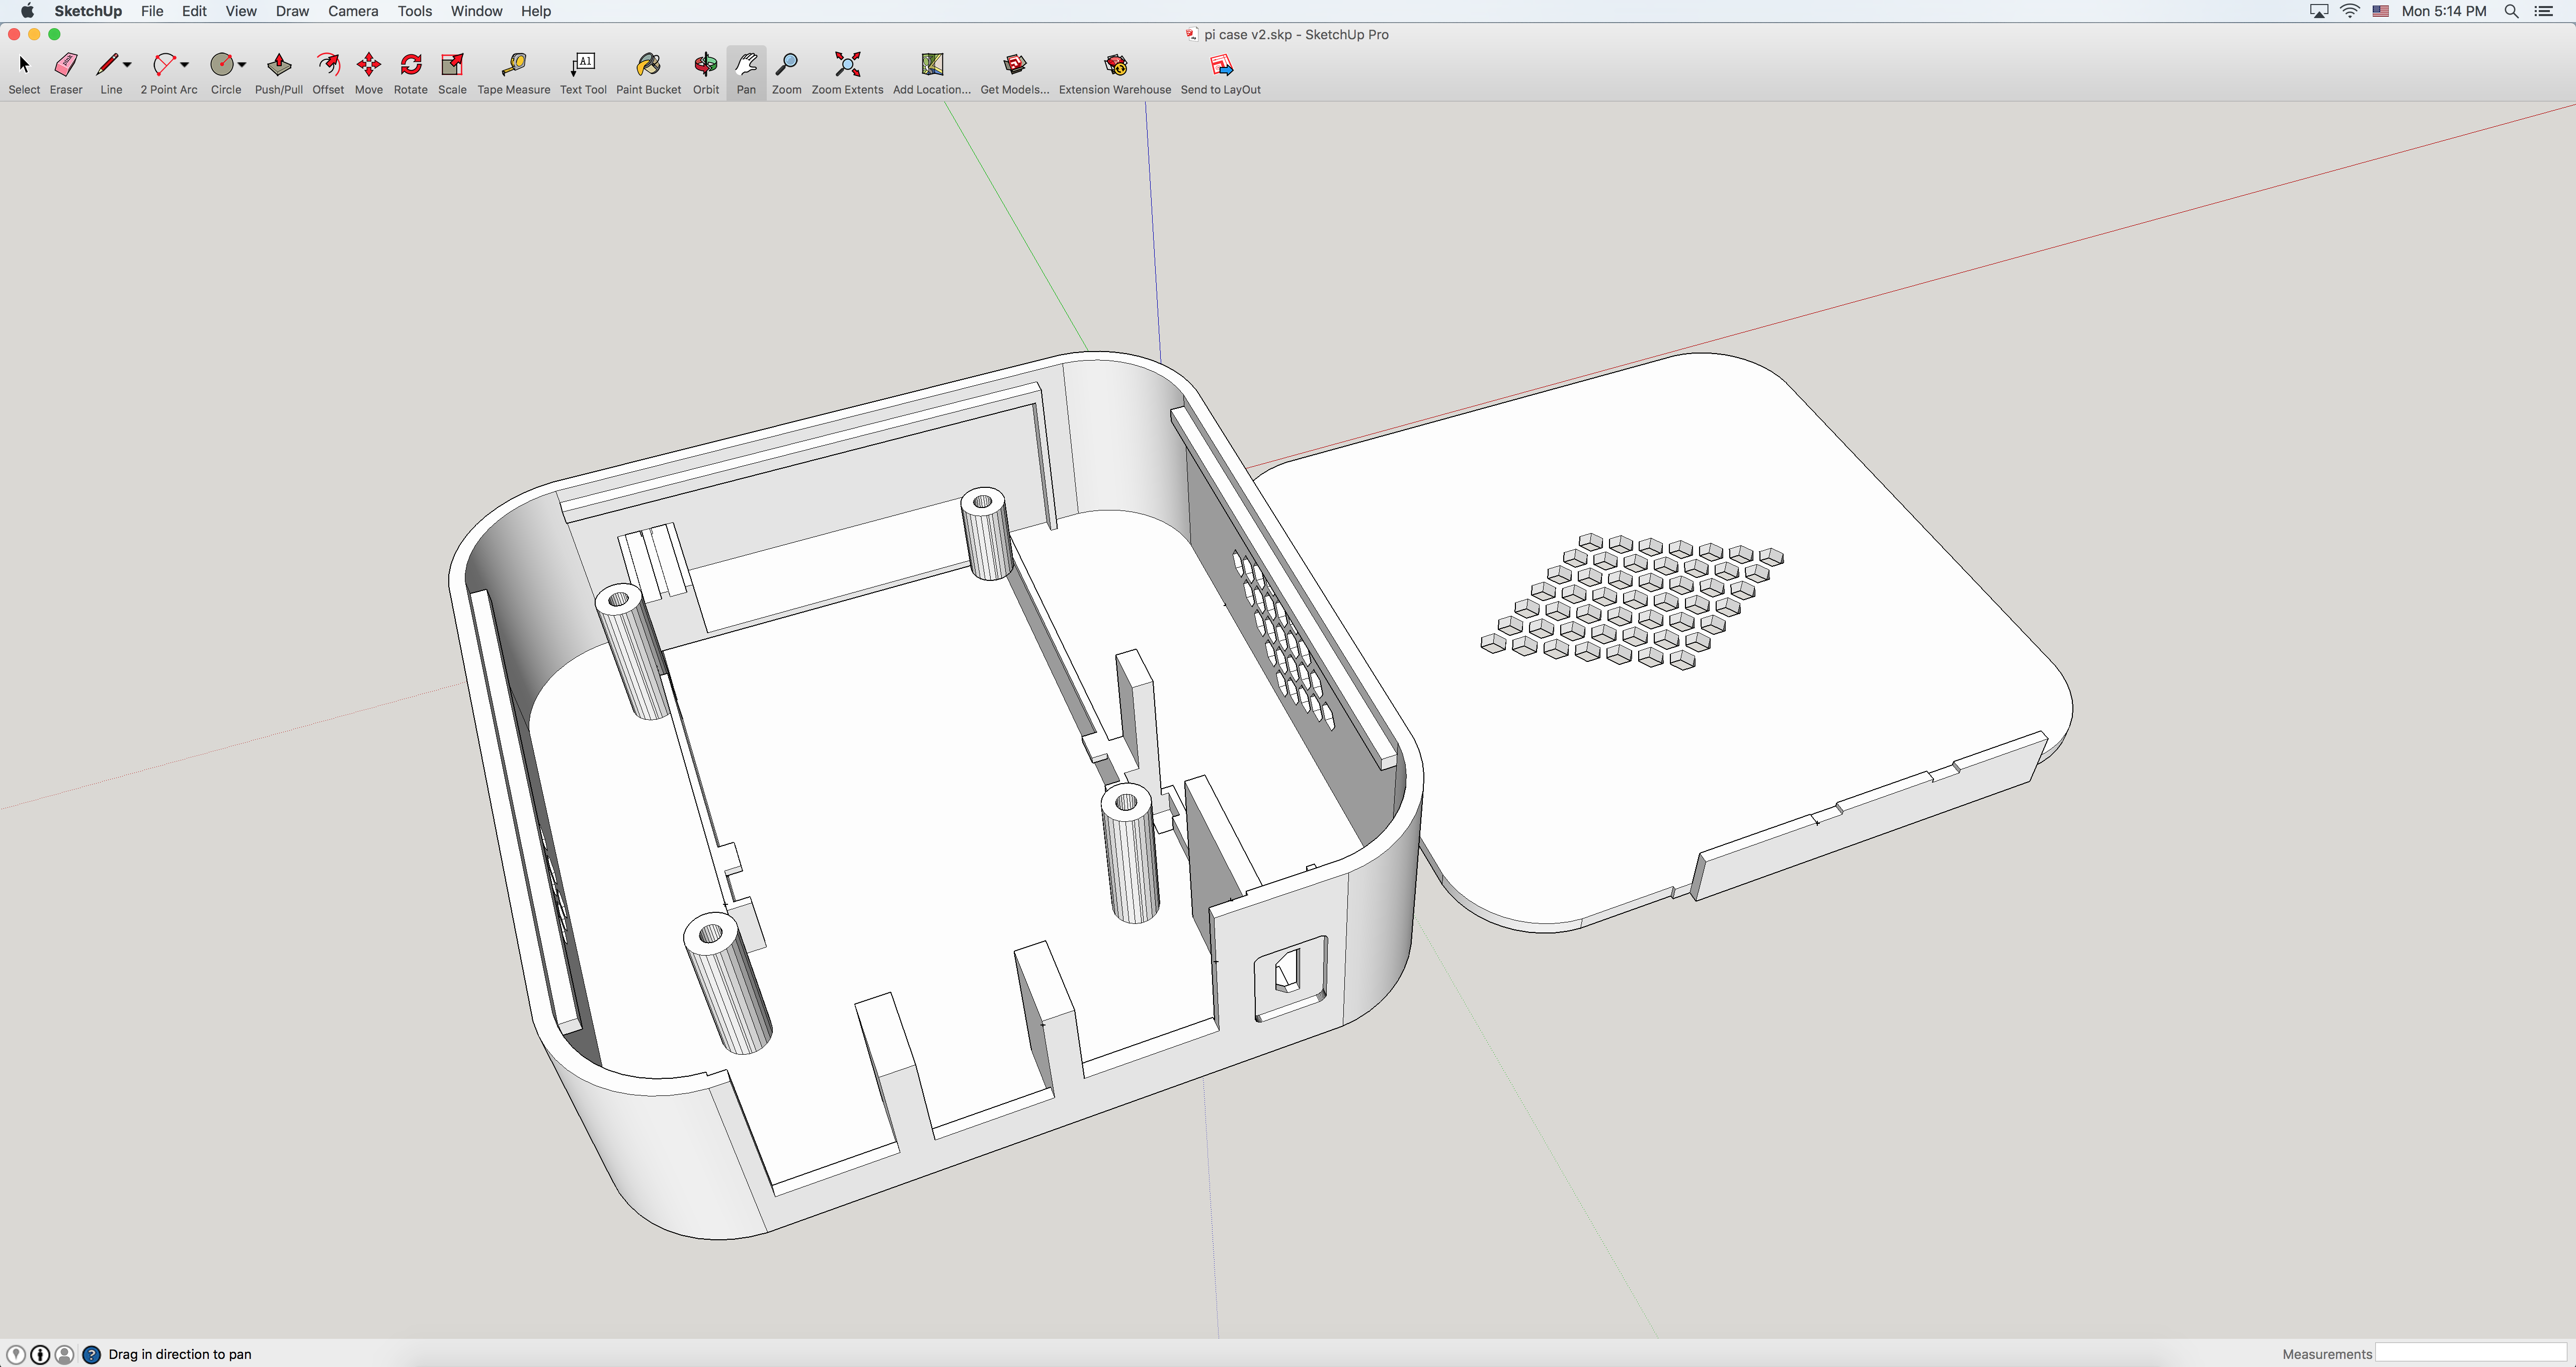
\includegraphics[width=8cm]{./images/V2.png}
		\caption{Pi Case Version1 and Version2}
	\end{figure}
\end{center}
\begin{center}
	\begin{figure}[h]
		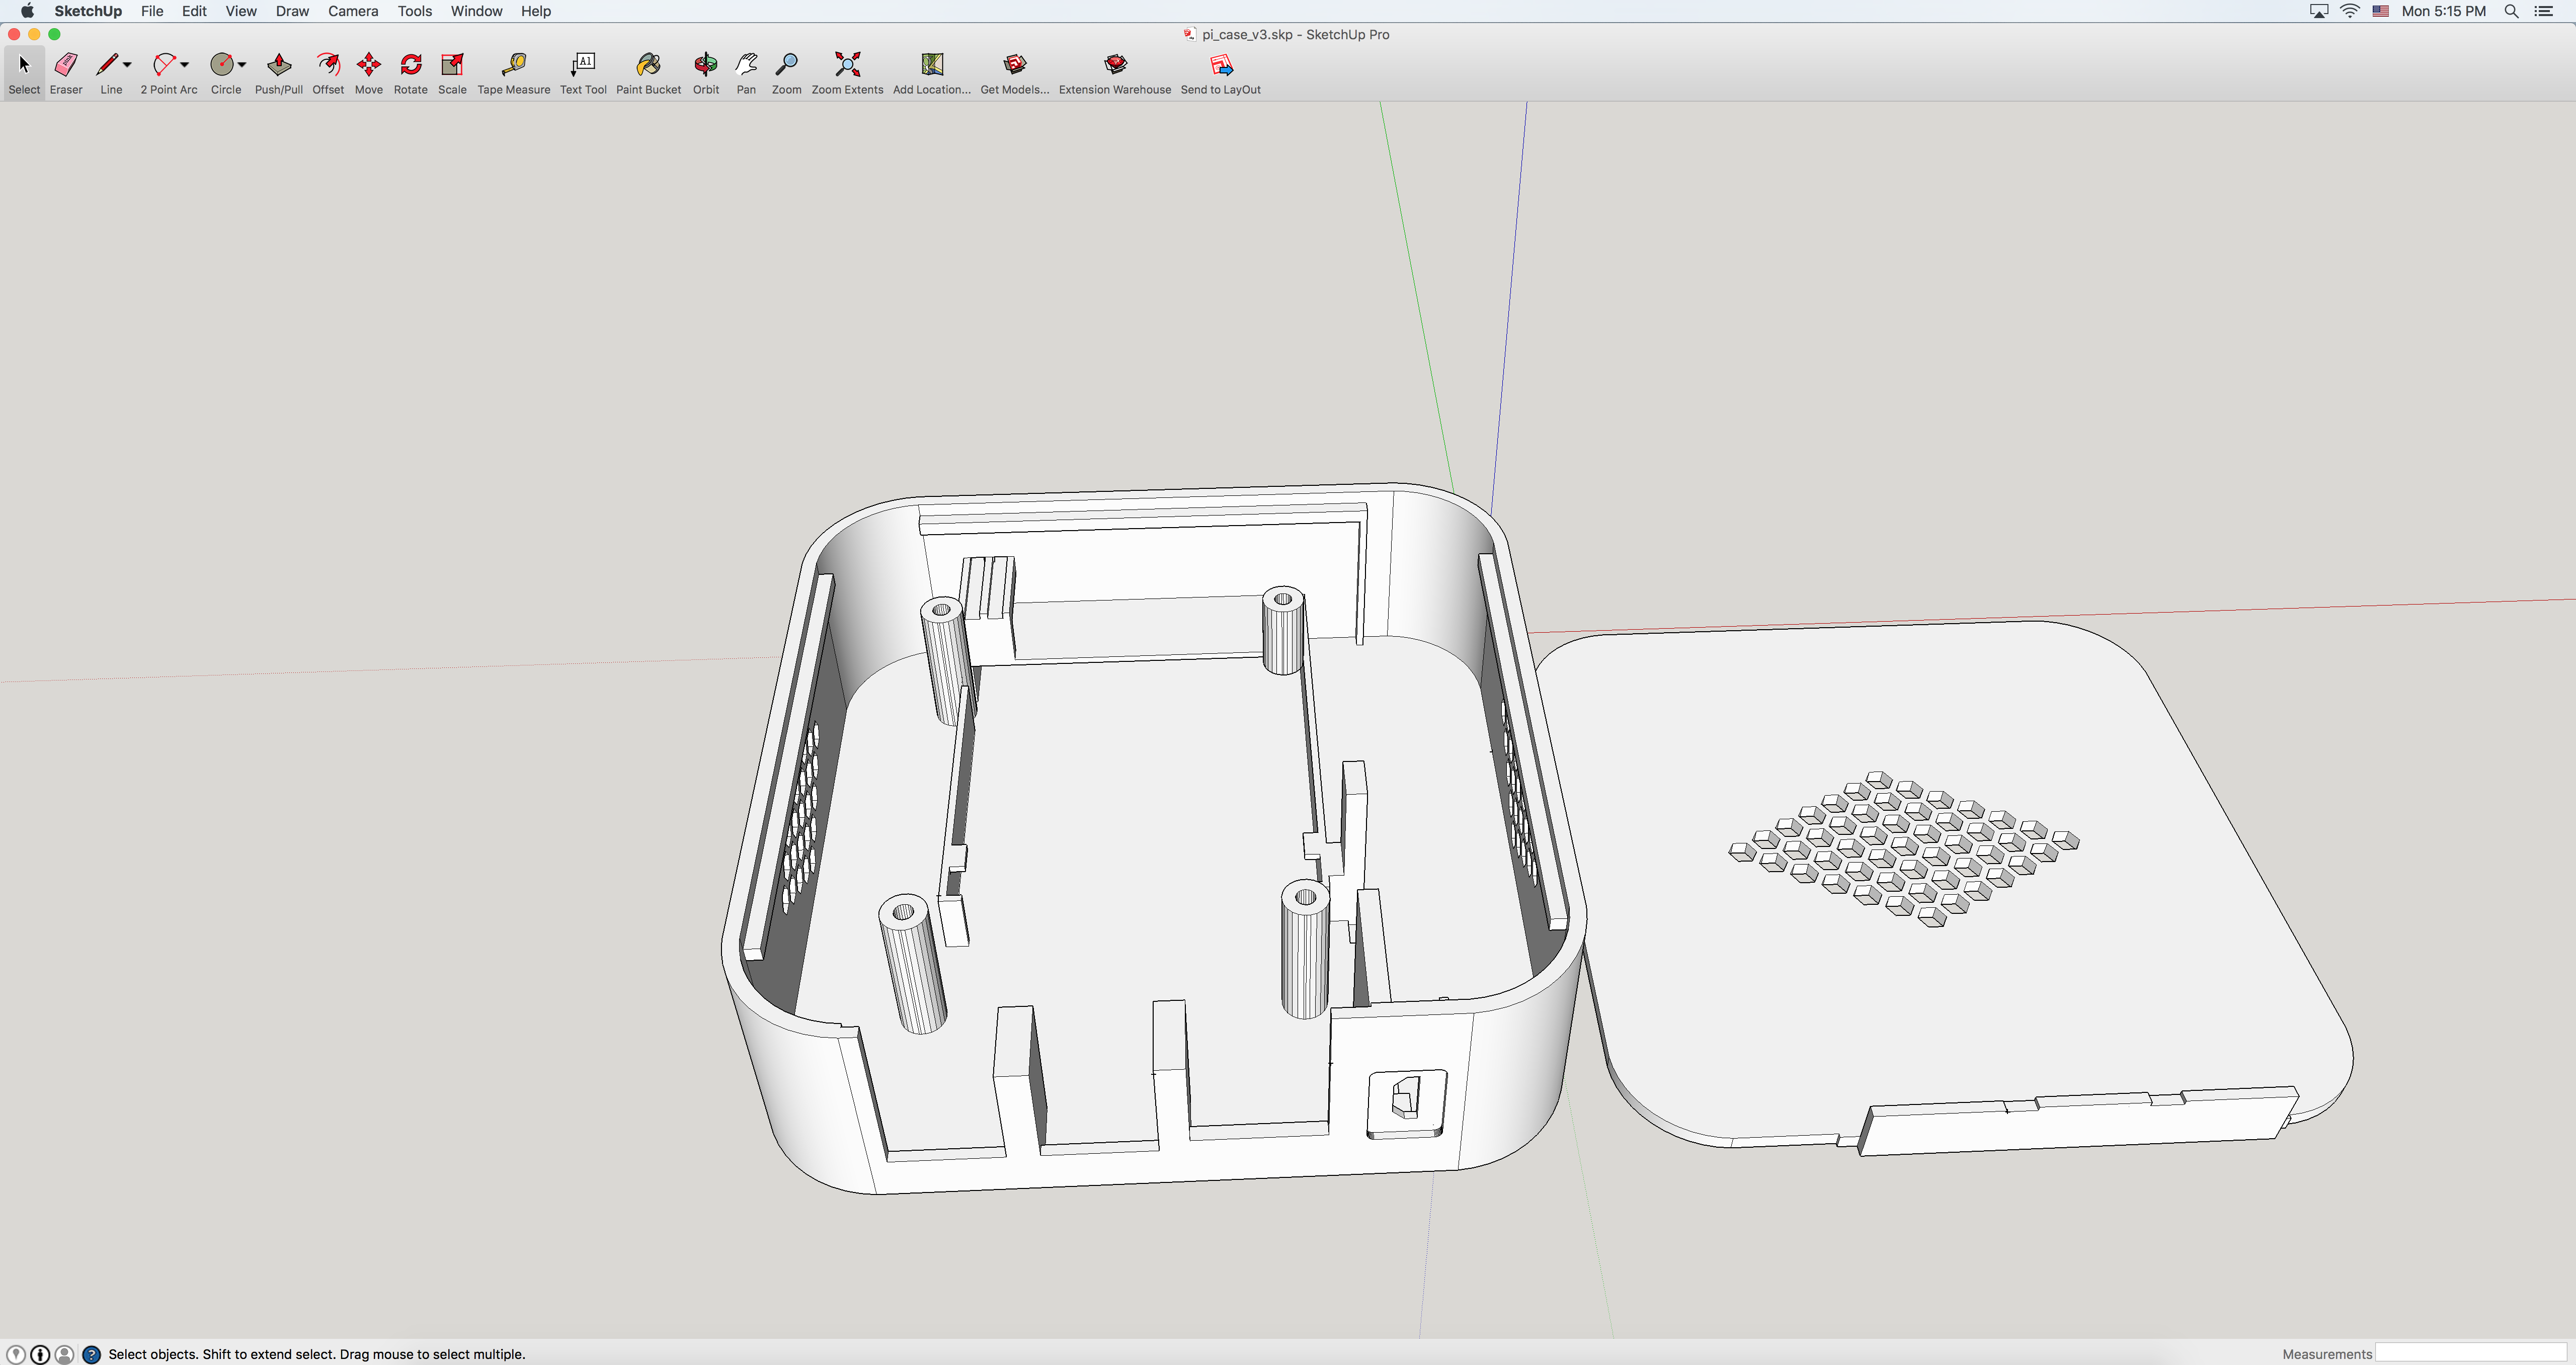
\includegraphics[width=8cm]{./images/V3.png}
		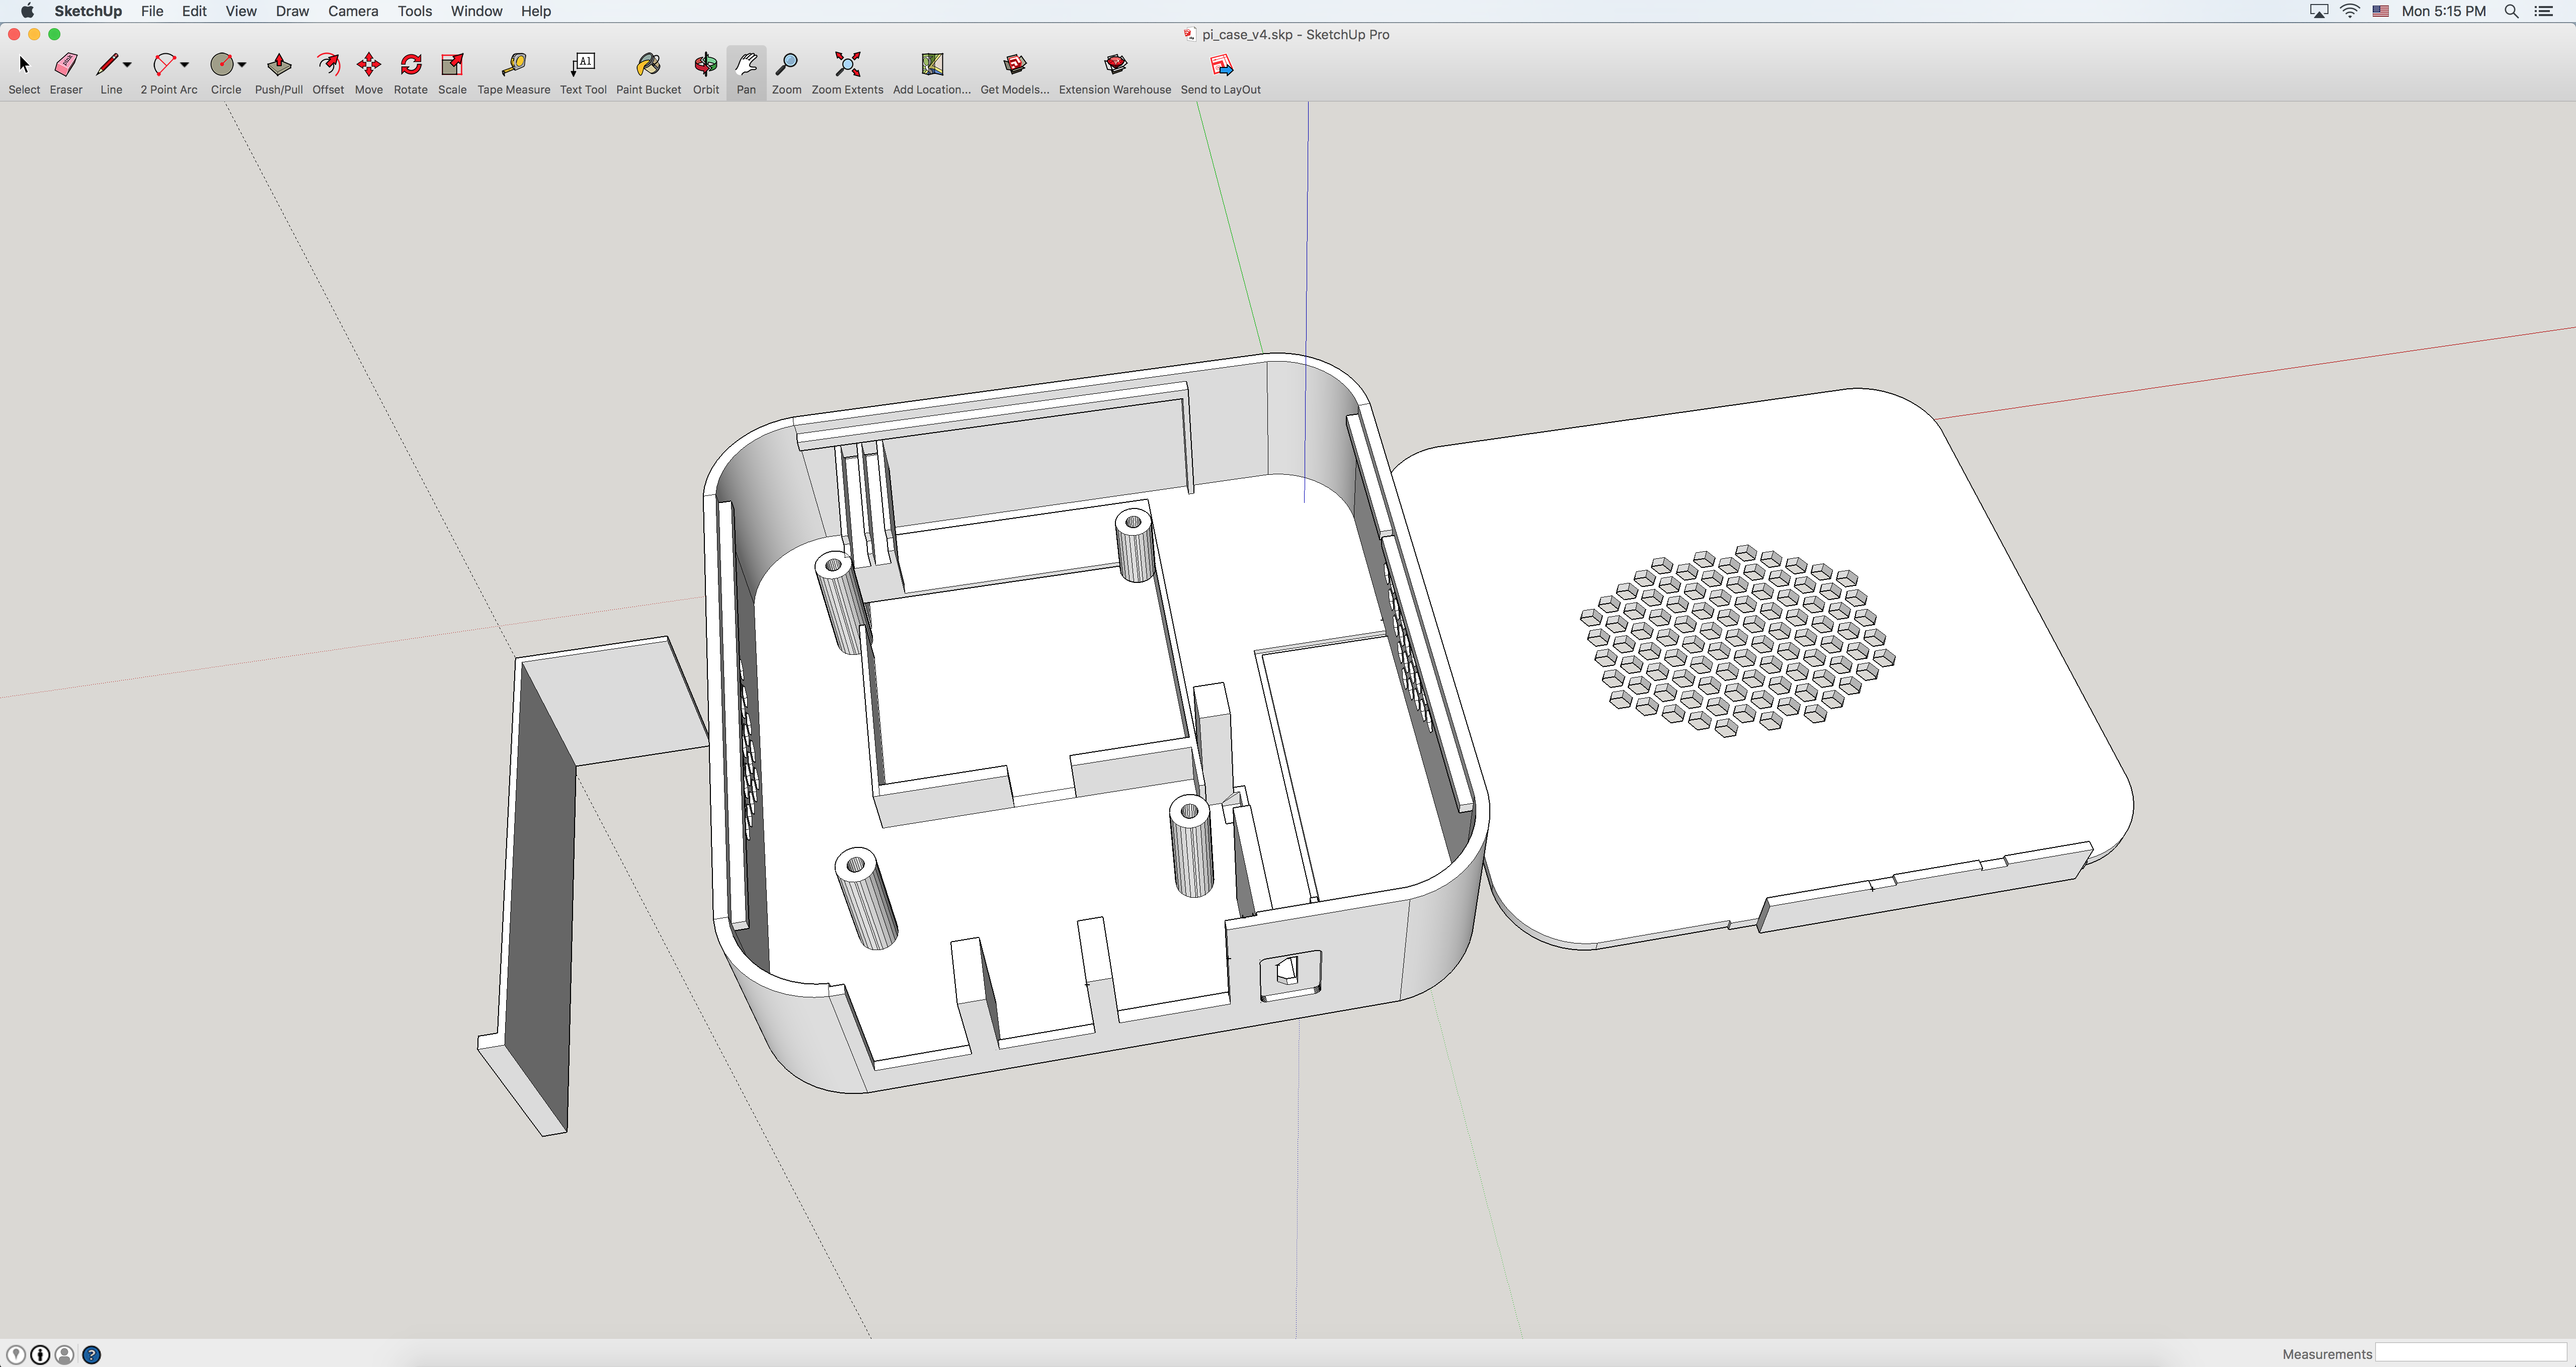
\includegraphics[width=8cm]{./images/V4.png}
		\caption{Pi Case Version3 and Version4}
	\end{figure}
\end{center}
Pi 케이스 V3은 일체형으로 3D 프린팅을 하여 리튬이온 배터리 장착부분의 지지대가 잘 제거되지 않고 지지대를 제거 하더라도 조금의 잔여물이 남아 배터리가 찌그러지는 현상이 발생하였다. 그리고 전원부분의 구멍이 딱맞지 않아 오른쪽으로 0.3mm, 밑으로 0.2mm 조정하였다. 또 파이의 열이 온습도 센서로 바로 가서 보통의 센서 보다 온도는 높게 그리고 습도는 낮게 표시 되었다. 이를 해결해 주기위해서 격벽을 만들어 주었고 케이블 수납 공간이 부족하여 케이스 크기를 가로 세로 1cm 씩 늘렸다.
Pi 케이스 V4는 마지막에 전원 선연결이 쉽지 않은 문제점이 있었다.
\begin{center}
	\begin{figure}[h]
		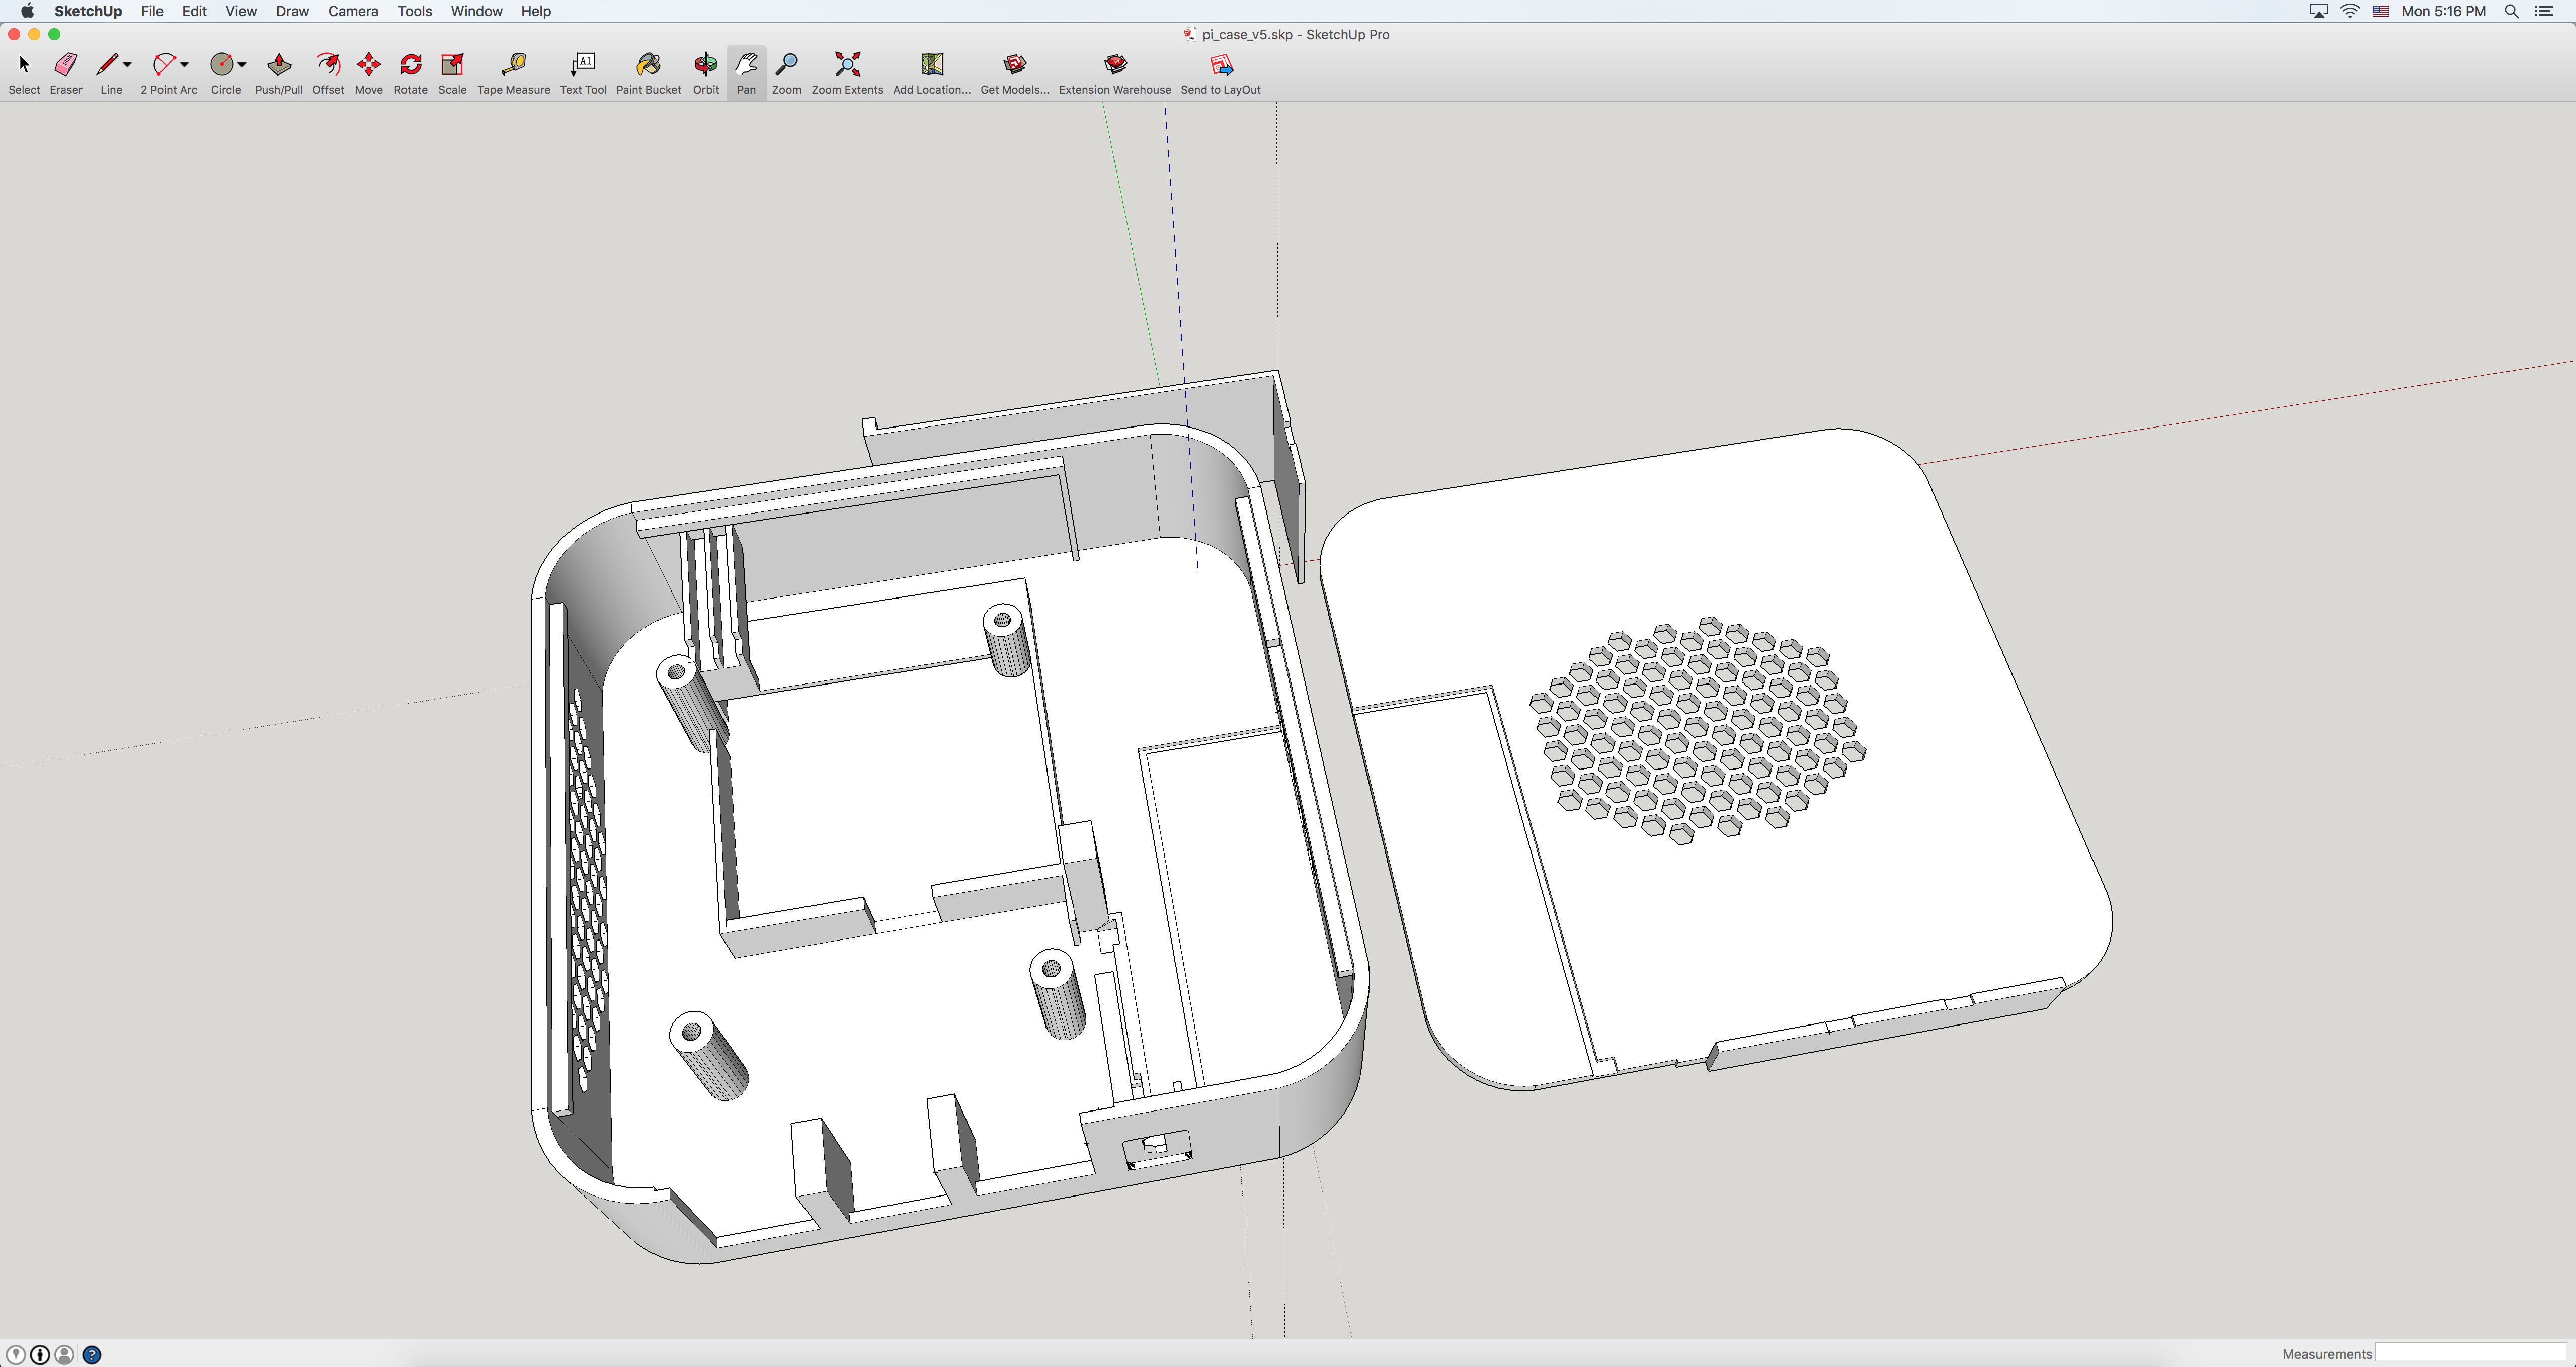
\includegraphics[width=8cm]{./images/V5.png}
		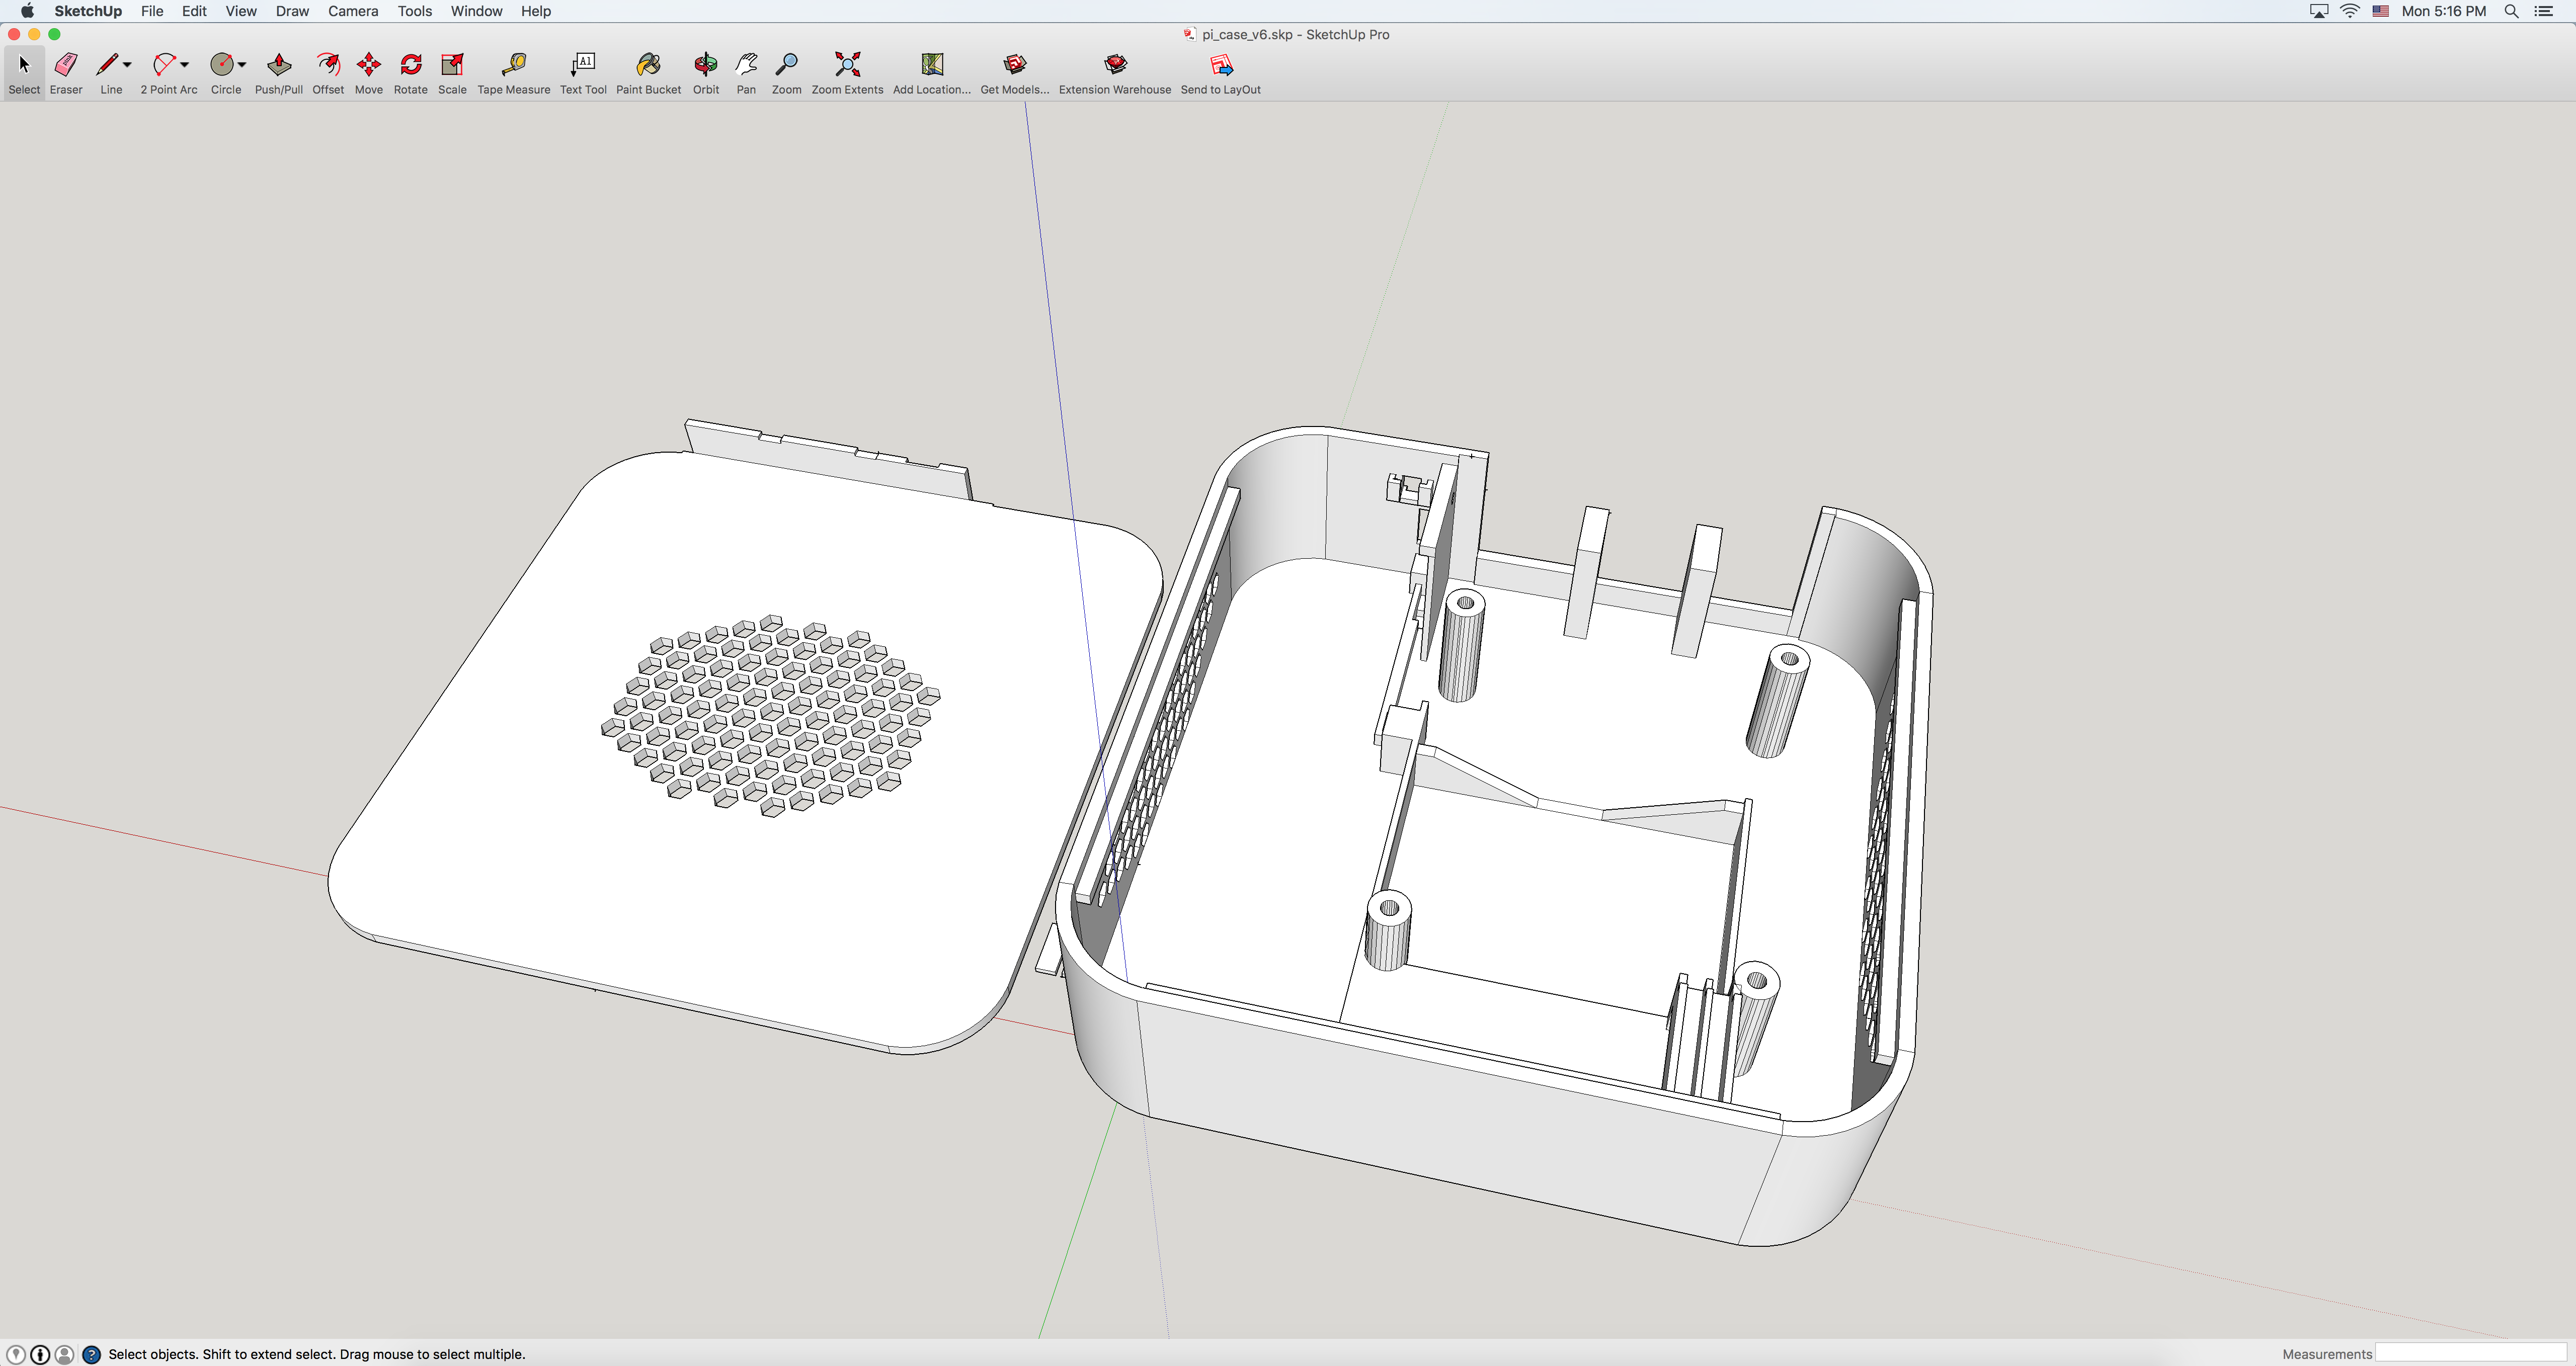
\includegraphics[width=8cm]{./images/V6.png}
		\caption{Pi Case Version5 and Version6}
	\end{figure}
\end{center}
\begin{figure}[h]
	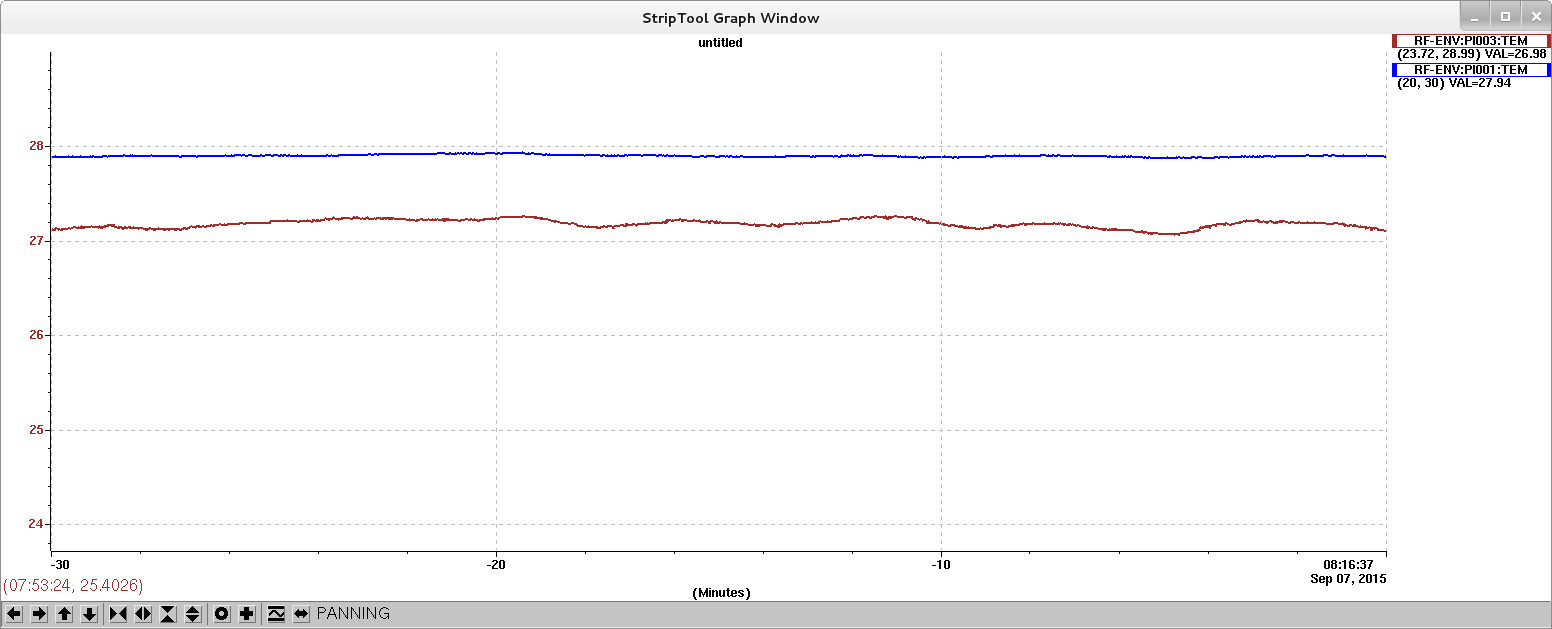
\includegraphics[width=10cm]{./images/65.png}
	\caption{Striptool을 이용한 RF-ENV:PI002:TEM와 RF-ENV:PI003:TEM의 plot}
\end{figure}

케이스 안에 들어있는 센서와 밖으로 빼놓은 센서는 눈으로 보기에는 1도 정도의 차이를 가졌고 이를 확실하게 확인하기 위해서 통계 프로그램 R을 이용해 확인하였다. 메뉴얼에 나와있는 센서의 오차범위는 0.4도 이므로 정규 분포화 했을때 온도가 이 오차범위 이내로 들어온다면 괜챃을 것이라고 판단하였다.
\begin{center}
	\begin{figure}[h]
		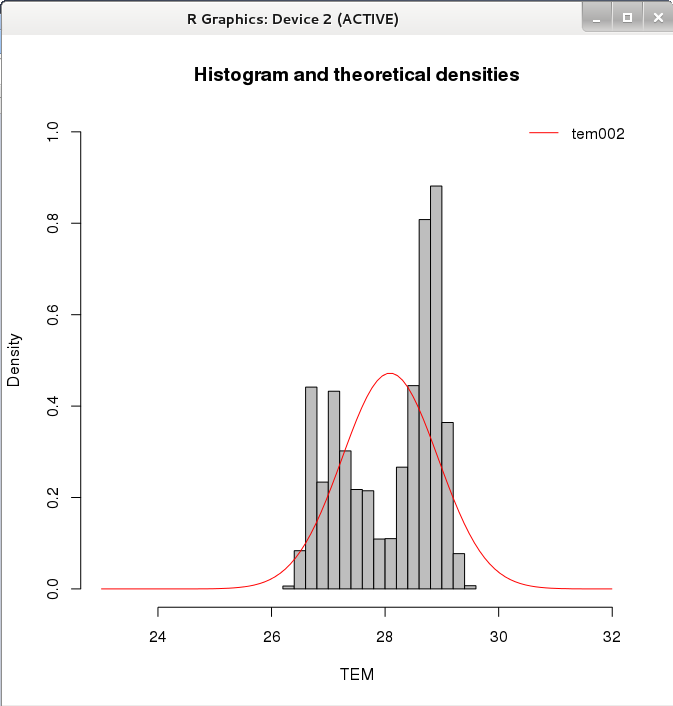
\includegraphics[width=7cm]{./images/R1.png}
		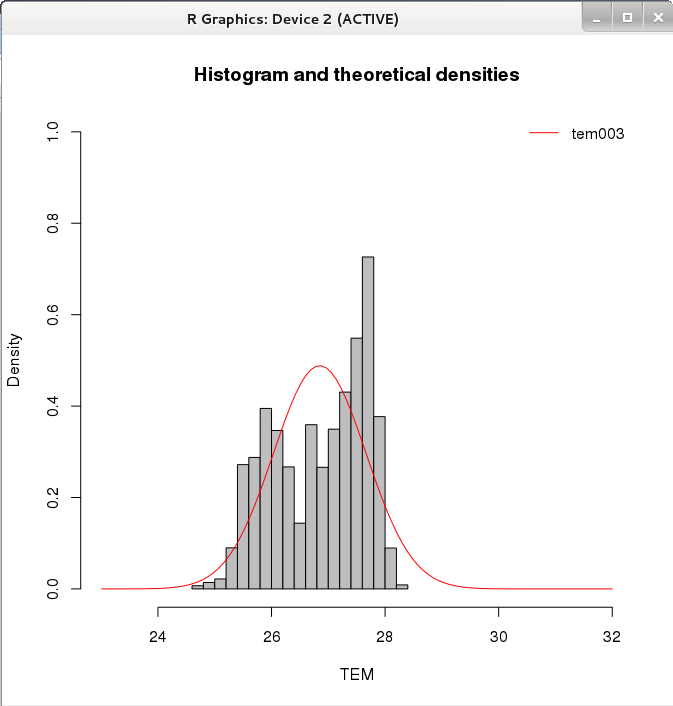
\includegraphics[width=7cm]{./images/R2.png}
		\caption{RF-ENV:PI002:TEM와 RF-ENV:PI003:TEM의 정규분포 그래프}
	\end{figure}
\end{center}

두개의 정규분포 그래프의 bin수 등 모든 조건을 일치시킨 상태에서 정규분포화 시켰으며 60000개 이상의 데이터를 샘플링하였다.

\begin{center}
	\begin{figure}[h]
		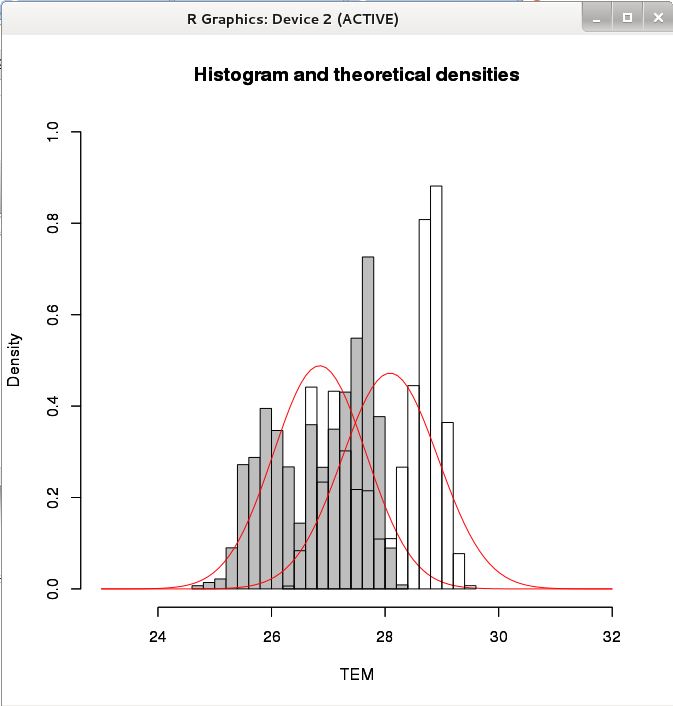
\includegraphics[width=7cm]{./images/rtest1.png}
		\caption{RF-ENV:PI002:TEM와 RF-ENV:PI003:TEM의 정규분포 그래프}
	\end{figure}
\end{center}
\begin{center}
	\begin{figure}[h]
		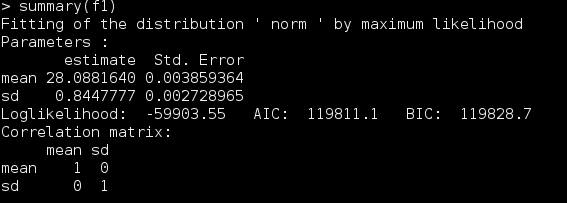
\includegraphics[width=7cm]{./images/16.png}
		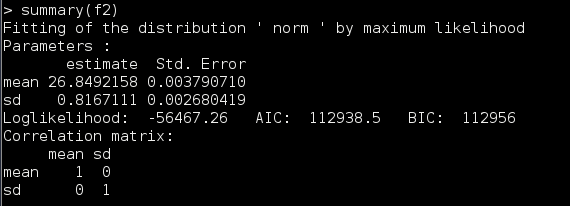
\includegraphics[width=7cm]{./images/74.png}
		\caption{RF-ENV:PI002:TEM와 RF-ENV:PI003:TEM}
	\end{figure}
\end{center}
확인해본 결과 두 센서의 mean 값 차이는 1.05도 정도로 Pi 케이스 V5에서 파이의 열과 led로 인해 발생하는 열의 배출이 잘 이루어 지지 않는다고 판단해서 파이 아래 부분의 구멍을 좀더 크게 만들어 주었다.
Pi 케이스 V6는 리튬이온 배터리의 착탈착을 좀더 쉽게하기 위해서 배터리 격벽의 높이를 좀더 낮춰주고 사선으로 만들어서 착탈착을 쉽게 만들어 주었다.

\begin{center}
	\begin{figure}[h]
		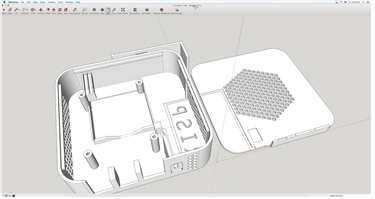
\includegraphics[width=7cm]{./images/V7.png}
		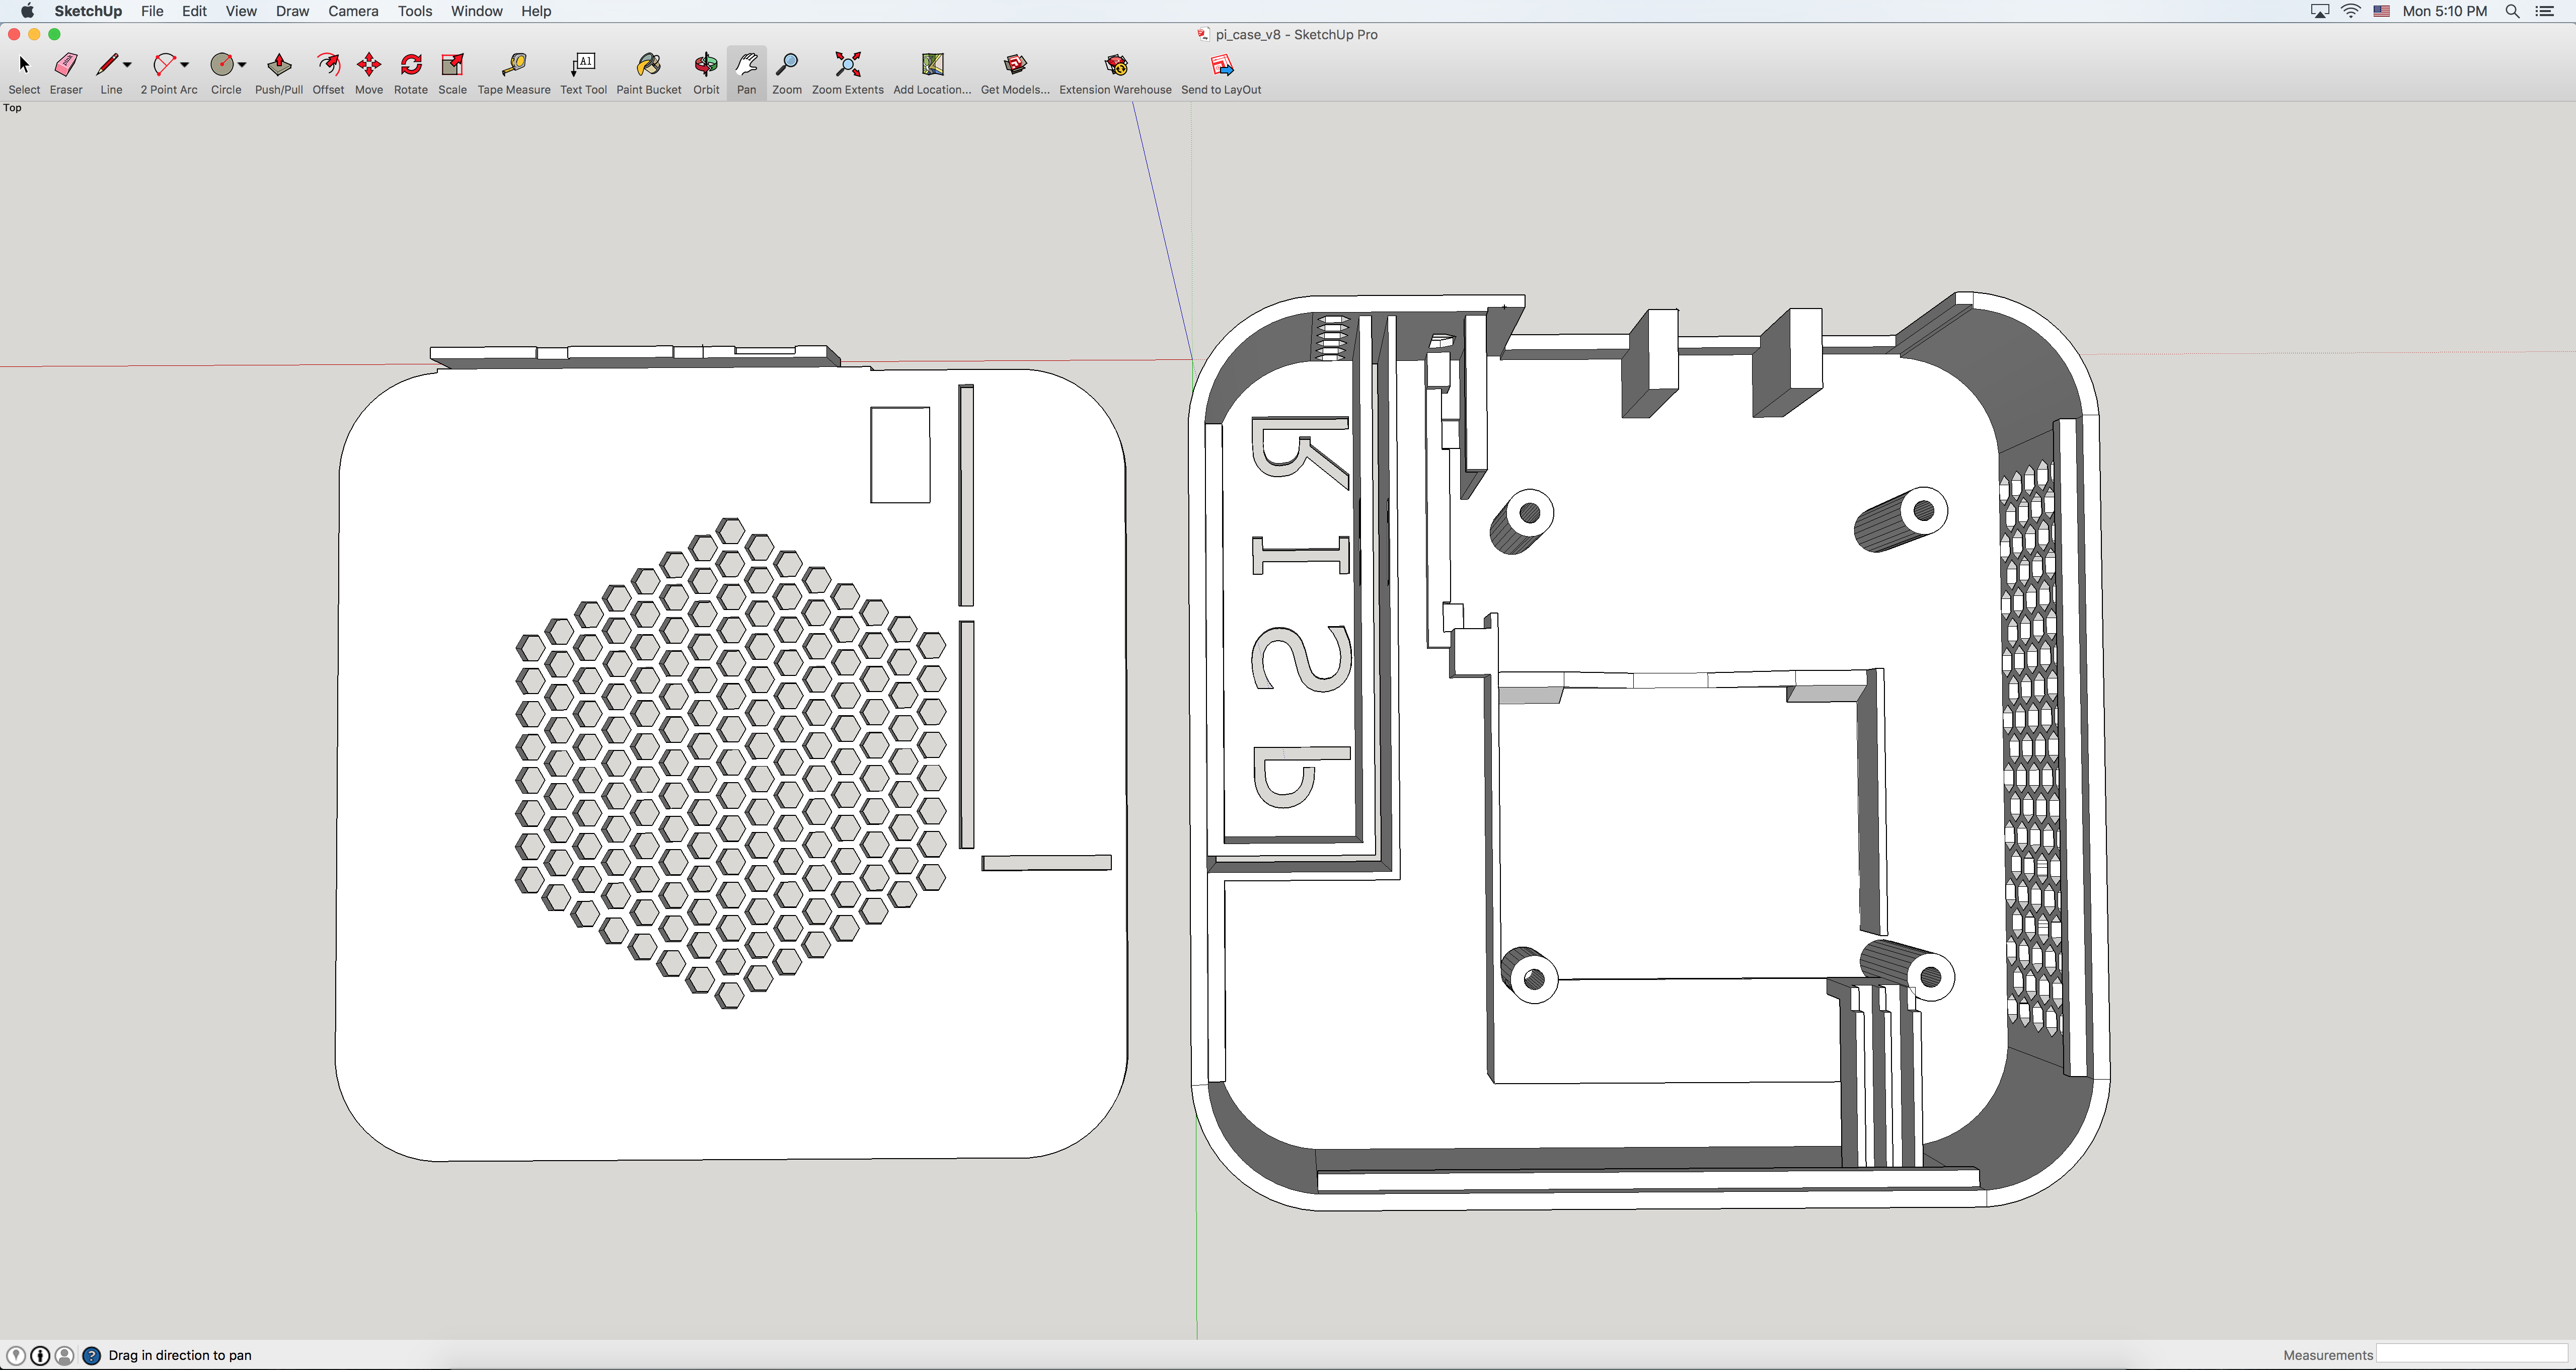
\includegraphics[width=7cm]{./images/V8.png}
		\caption{Pi Case Version7 and Version8}
	\end{figure}
\end{center}
\begin{center}
	\begin{figure}[h]
		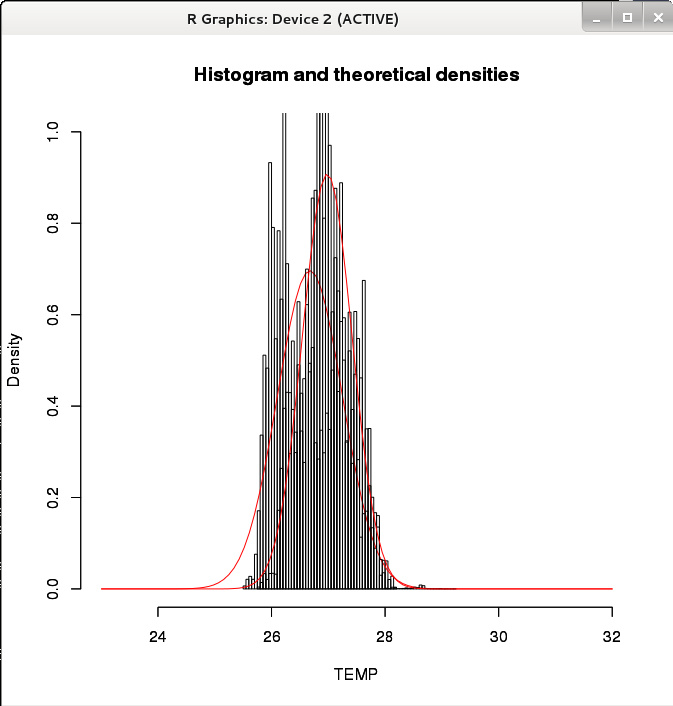
\includegraphics[width=7cm]{./images/R.png}\\
		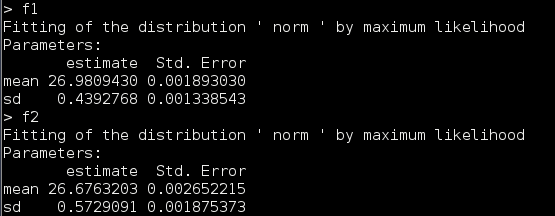
\includegraphics[width=7cm]{./images/157.png}
		\caption{RF-ENV:PI002:TEM와 RF-ENV:PI003:TEM의 정규분포 그래프}
	\end{figure}
\end{center}
아래의 R을 통해서 만든 정규 분포표를 보면 안과 밖 두 센서의 평균값이 0.3도 정도의 차이를 보이므로 이 케이스를 사용하기로 하였다.
Pi 케이스 V7은 위쪽과 옆쪽 으로도 많은 열 배출구를 많들어 파이가 빨리 식을수 있도록 만들었다. 그리고 센서가 들어가는 부분도 위와 옆부분의 구멍을 만들어 바람이 잘 통할수 있는 상황을 만들어 주었다.
\clearpage
\chapter{Pi와 Pi Case 조립 및 설치}
\section{Pi와 Pi Case 조립}
\begin{center}
	\begin{figure}[h]
		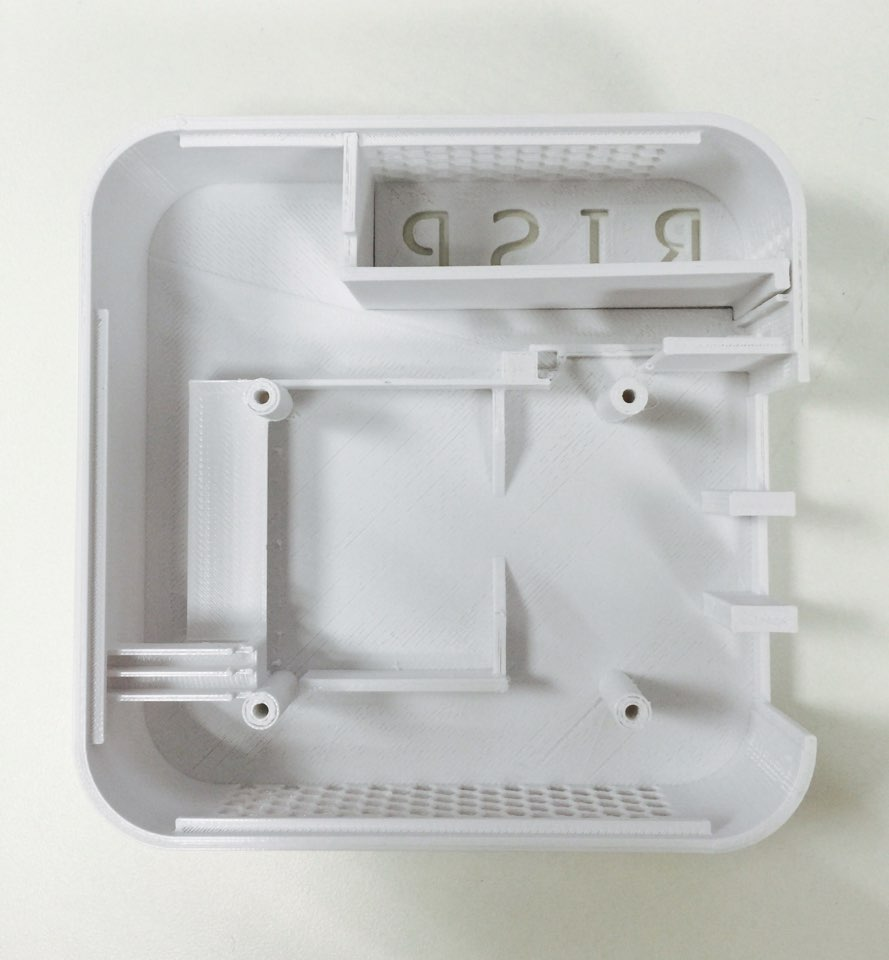
\includegraphics[width=5cm]{./images/a.jpg}
		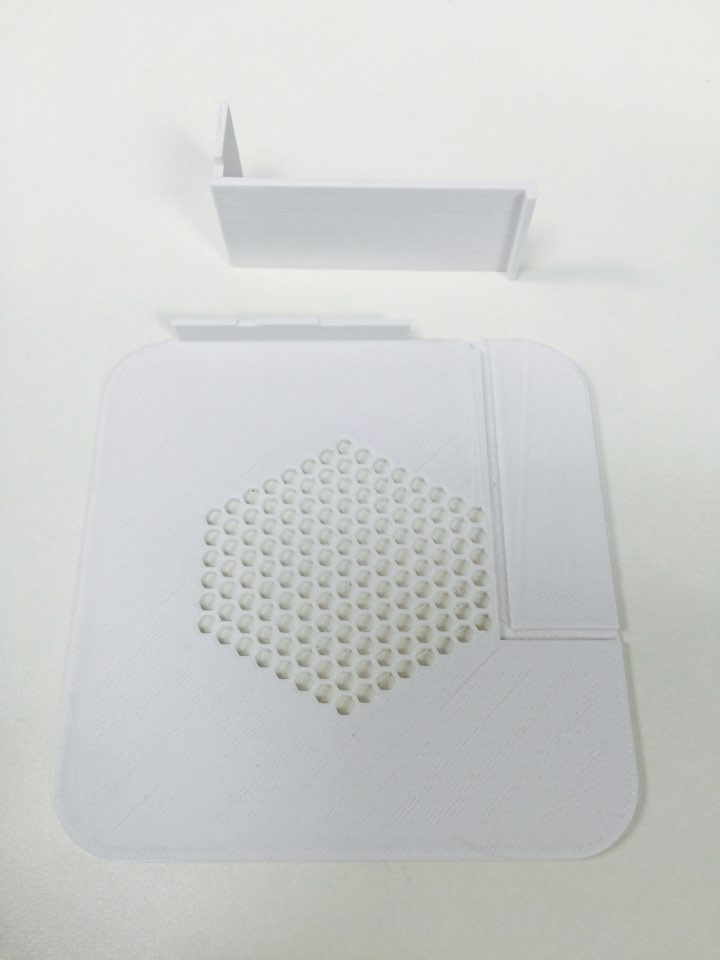
\includegraphics[width=4.1cm]{./images/b.jpg}
		\caption{상판과 하판 및 격벽}
	\end{figure}
\end{center}
\begin{center}
	\begin{figure}[h]
		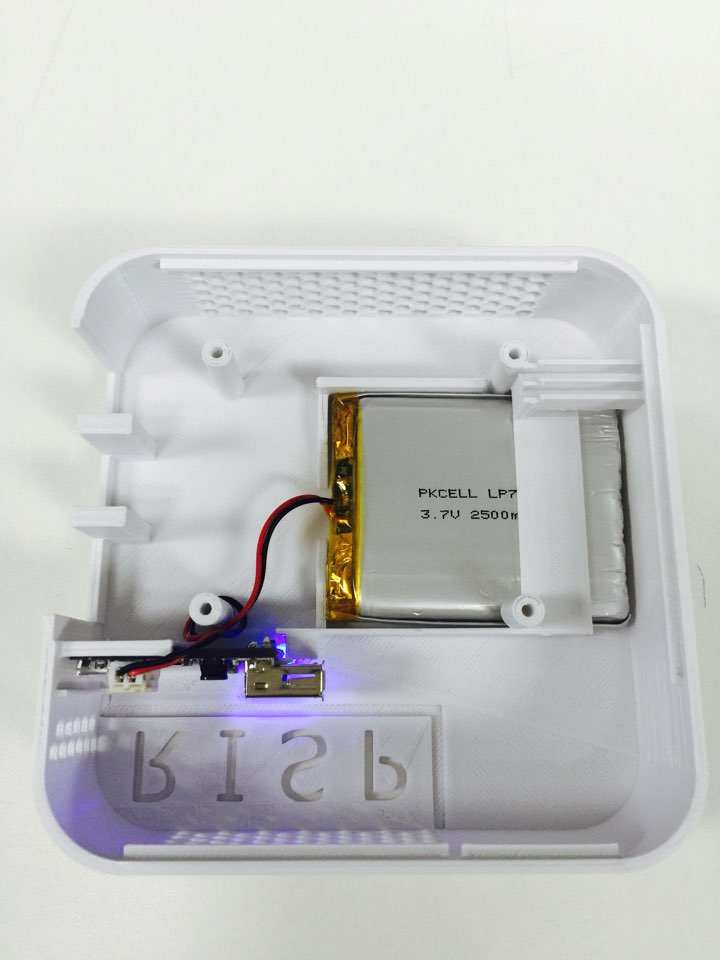
\includegraphics[width=4.1cm]{./images/c.jpg}
		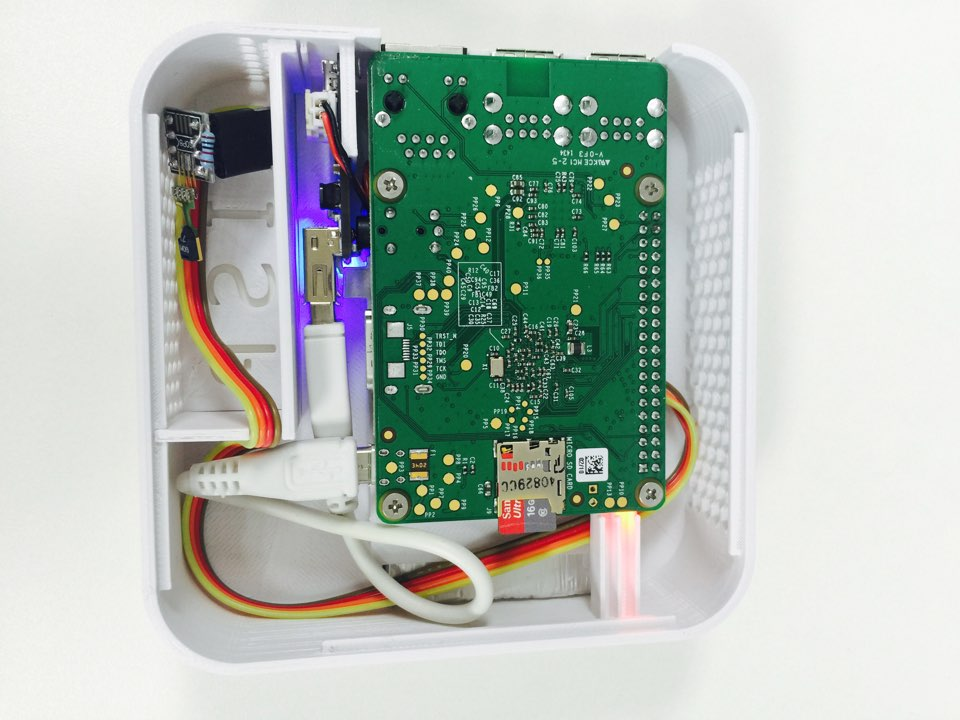
\includegraphics[width=7.2cm]{./images/f.jpg}
		\caption{UPS와 완전 조립 모습}
	\end{figure}
\end{center}
PowerBoost unit과 리튬이온 배터리를 이용해서 무정전 전원 공급장치를 만들었으며 케이스 내부에서 케이블이 꼬이지 않도록 케이블 정리를 하였다.
\clearpage
\begin{center}
	\begin{figure}[h]
		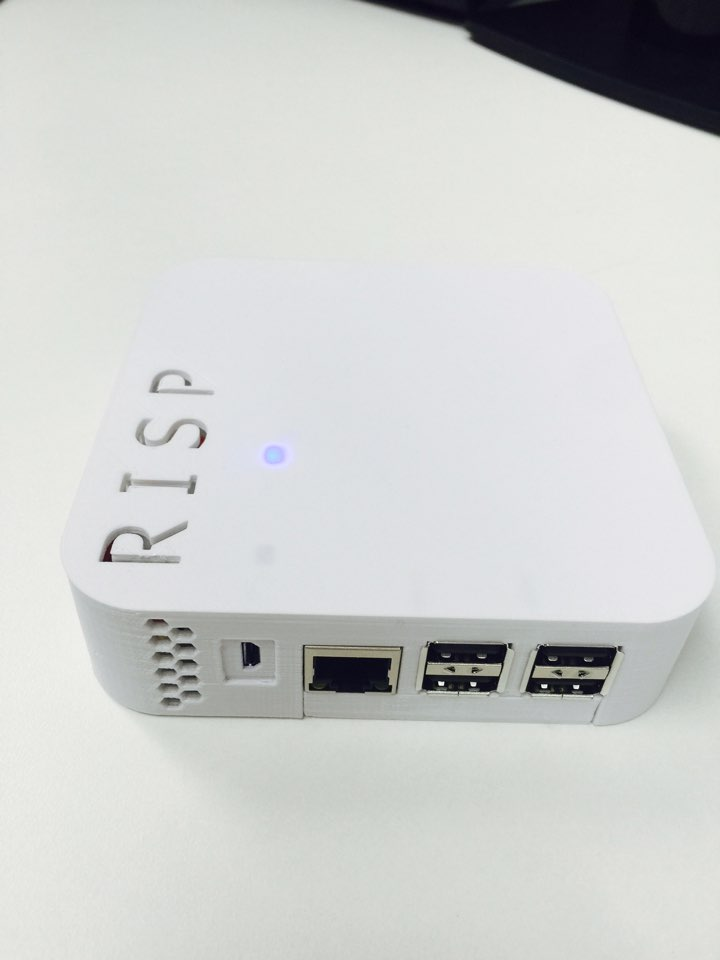
\includegraphics[width=4.5cm]{./images/d.jpg}
		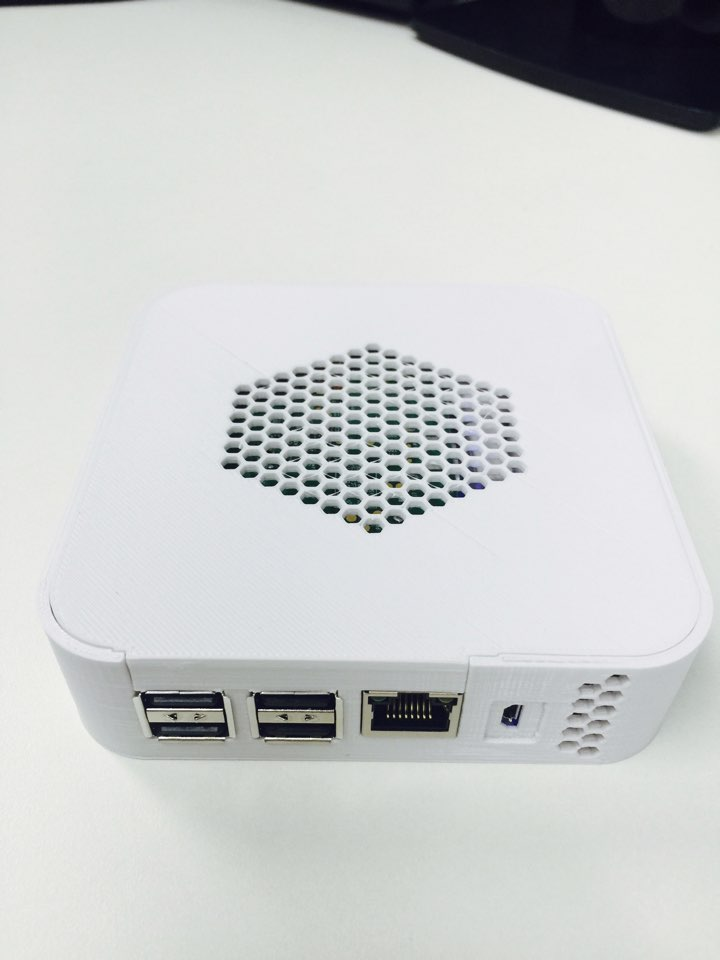
\includegraphics[width=4.5cm]{./images/e.jpg}
		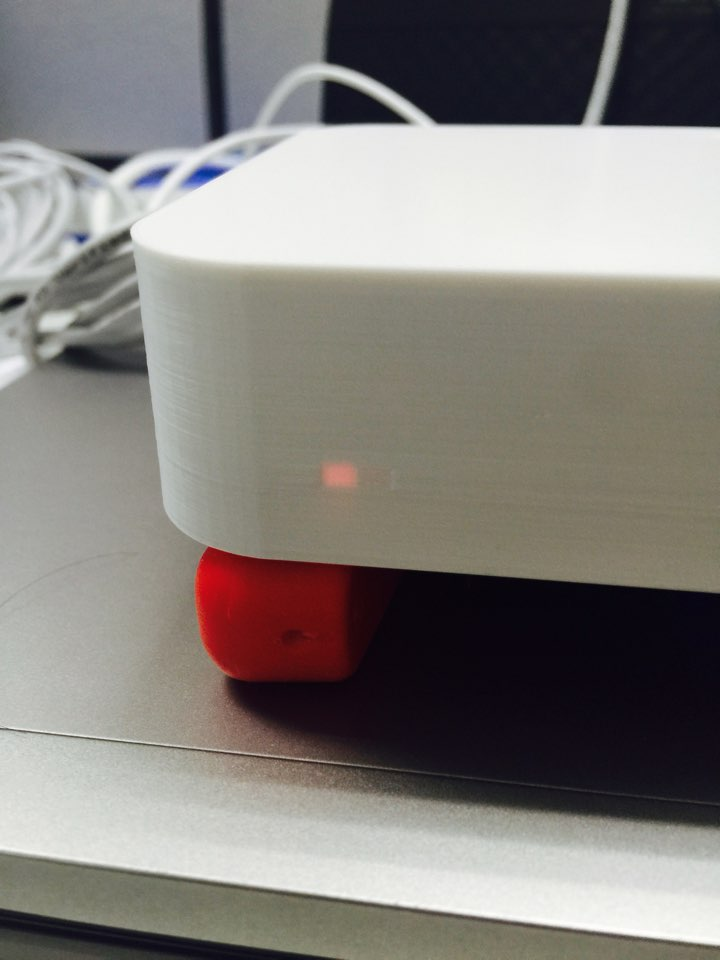
\includegraphics[width=4.5cm]{./images/g.jpg}
		\caption{완전 조립된 케이스}
	\end{figure}
\end{center}
전원공급 상황은 RISP글자 밑 파란 LED를 통해서 알수 있고 배터리 충전시에는 파란 LED 옆은 주황 LED로 알수 있다. 또 전면의 빨간 LED를 통하여 Pi의 작동상황을 알수 있도록 하였다.
\section{설치}
\begin{center}
	\begin{figure}[h]
		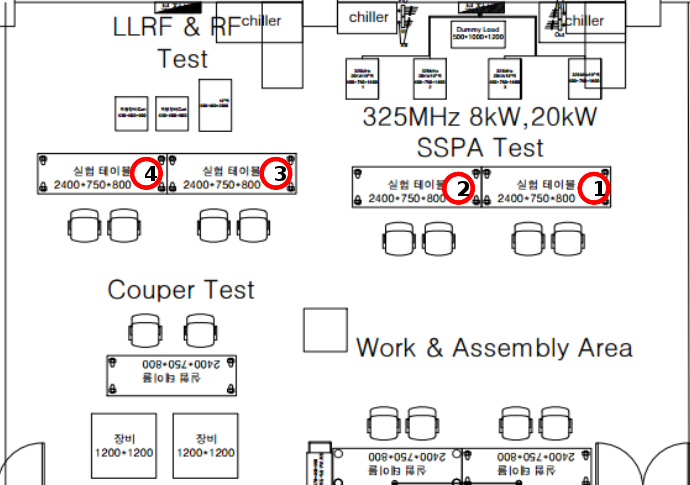
\includegraphics[width=8cm]{./images/RF.png}
		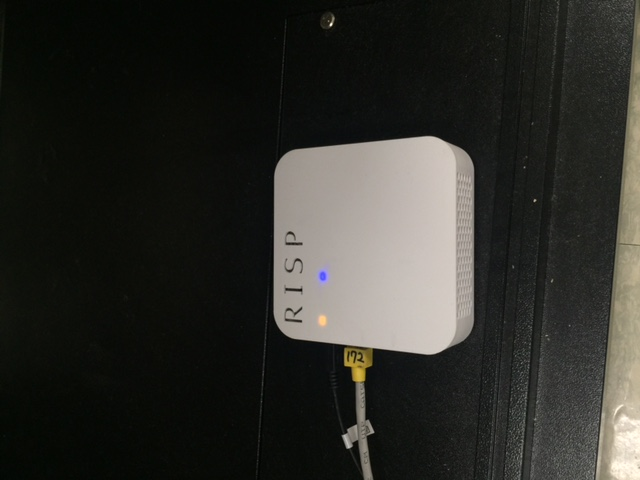
\includegraphics[width=7.5cm]{./images/72.JPG}
		\caption{환경모니터링용 Pi 설치 위치}
	\end{figure}
\end{center}
현재 2번 위치쯤에 파이가 설치되어 있으며 RF실험실의 실험환경이 다 꾸며 지지 않은 관계로 1개의 파이만 설치되어있는 상황이다 차후 실험실 환경이 다 갖추어지면 나머지 파이들도 설치될 예정이다.
\end{document}
